\section{Operating Instructions}

\subsection{General Information}
All operational controls and configurations are conveniently carried out from the front panel.

The two-line-by-40-characters LCD display, in conjunction with 4 cursor keys and an \EXECUTE button, allows easy and intuitive operation of the PT5300 HD-SD Varitime\TM Sync Generator.

The cursor keys are used to call relevant menus on the display: the top line of the display shows the current status/selection or other current menu choices.

In the upper right corner of the display is an indication of cursor keys used in the active menu.
\begin{itemize}
\item a \rightbuttontext  indicate that the right arrow buttons can be used
\item a \upbuttontext  indicates that the up button can be used
\item a \downbuttontext  indicates that the down button can be used
\item a \leftbuttontext  indicate that the left arrow buttons can be used
\item and an \execute  indicates that the \EXECUTE button can be used
\end{itemize}

The bottom line of the display indicates new selections or enables changes to parameter setting.

\subsection{Front Panel Controls}
\subsubsection{Navigation Key}
The circular key in the middle of the front panel is the so-called Navigation key or Compass key is the tool for making the navigation through the menus light and easy.

\textbf{Note:} The function of some of the output/input connectors on the rear panel depends upon the functional modules/options included your generator and the functional configuration.

\begin{figure}[hbt]
\centering
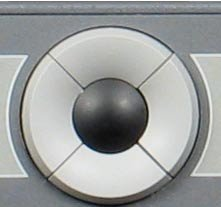
\includegraphics[width=0.2\textwidth]{fig/arrow_button}
\caption{PT5300 Navigation Keys}
\end{figure}

The black key in the middle is the \EXECUTE

The \upbuttontext (upper) button allows the user to exit the current menu and enter a higher-level menu, or to change parameter.

The \downbuttontext (lower) button allows the user to select new menus or sub-menus, or to change parameters.

The \leftbuttontext and \rightbuttontext (left and right) keys are used to scroll horizontally in the menus and to select the individual characters when naming presets an written text into the video full field test signals.

\paragraph{PRESET}
The \textbf{PRESET} button provides fast access to the instrument presets when switching between different standard applications.

\paragraph{OUTPUT}
The \textbf{OUTPUT} button provides a fast access to output signal selection on the generators.

\paragraph{GENLOCK}
The \textbf{GENLOCK} button provides a fast switching between locked and unlocked mode. The green LED next to the button indicates that \textbf{GENLOCK} has been selected. The type of genlock is selected via the menu.

\subsection{Indicators and Connections}
\subsubsection{Front Panel Indicators}
\paragraph{POWER ON}
A green LED that indicates when DC power is available from the internal DC supply.

\paragraph{WARNING}
A red LED indicates that the instrument has detected an irregularity. A more thorough description is given in the display. More errors if any can be found in the error log function.

\paragraph{UNLOCKED}
A red LED that indicates when genlock mode is enabled but no correct genlock signal is found on the active genlock input. In this case, the generator switches automatically to internal mode until a valid genlock signal becomes available.

\textbf{Note:} The function of some of the output/input connectors on the rear panel depends upon the functional modules/options included your generator and the functional configuration.

\begin{figure}[hbt]
\centering
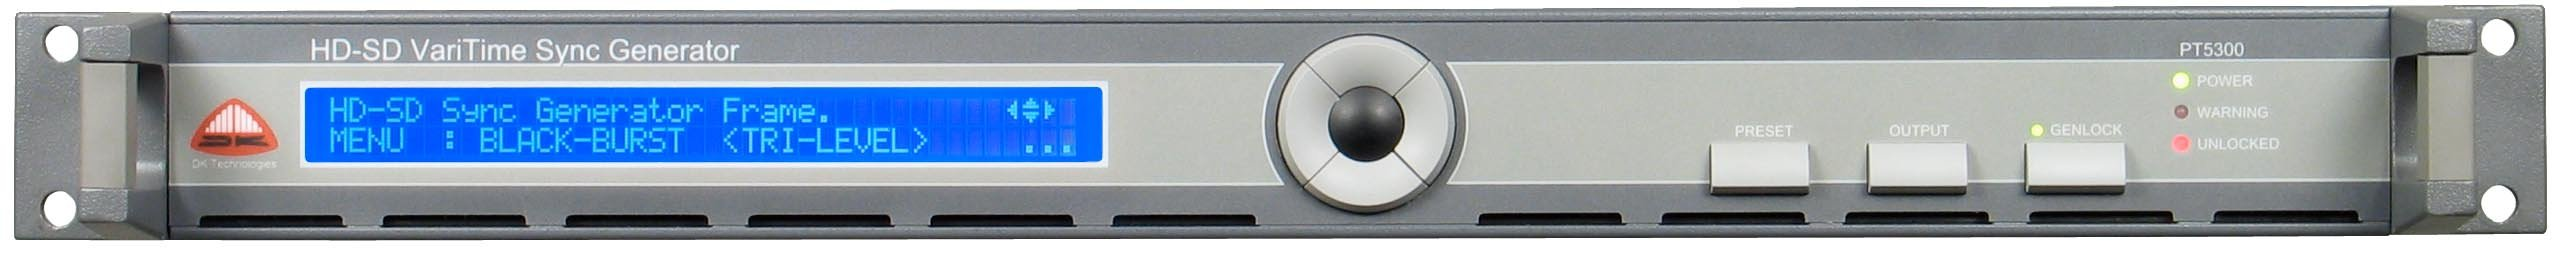
\includegraphics[width=0.8\textwidth]{fig/PT5300_front}
\caption{Front panel}
\end{figure}

\subsection{Display Information}
To guide the user through operations, symbols of the push buttons, which can be activated at a particular time will appear on the right side of the display.

\begin{tabular}{l p{41em}}
\upbuttontext \downbuttontext \leftbuttontext \rightbuttontext & Indicates which of the buttons in the Navigation are active \\
\execute &	Indicates that the \EXECUTE button (the black in the middle) must be pressed to activate the required selection \\
$< >$			& Indicates the position of the cursor on the menu line \\
$[$ $]$			& Indicates that changes to individual characters or digits are possible in timing and naming menus \\
\ldots		& Indicates that more items are available on the menu line \\
\locked		& Indicates that the panel is locked. Four different locked modes are available. The padlock will be only visible when the ``performed'' function is locked \\
\escape		& To abandon changes, place the cursor on \escape and press also \upbutton \\
\save			& To save a changed parameter, place the cursor on \save and press the \execute button \\
\end{tabular}

\subsection{Rear Panel Connections}

\textbf{Note:} The function of some of the output/input connectors on the rear panel depends upon the functional modules/options included your generator and the functional configuration.

\begin{figure}[hbt]
\centering
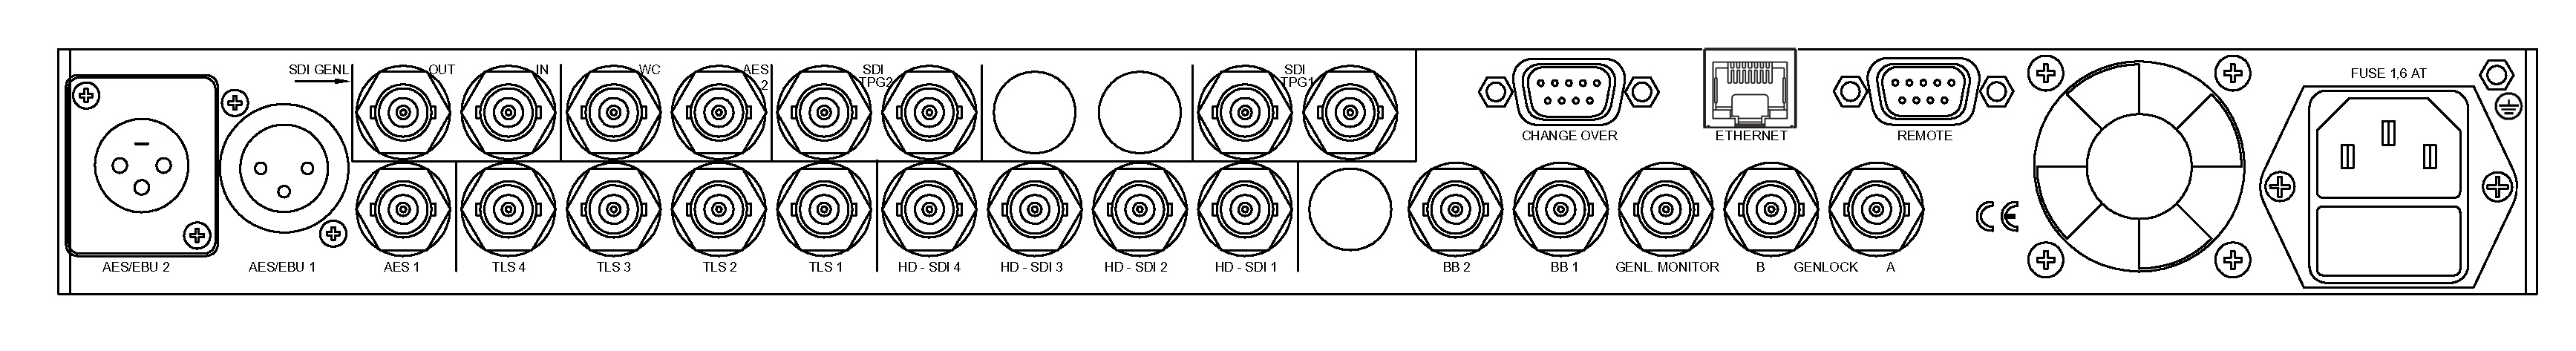
\includegraphics[width=\textwidth]{fig/PT5300_rear_view}
\caption{Rear panel}
\end{figure}

\textbf{Safety Ground (chassis)}


\includegraphics[width=2em]{fig/ground_symbol}

%\textbf{On/Off button}
%
%Mains switch
%
%\begin{tabular}{l l}
%ON:		& When ``I'' is pressed\\
%OFF:	& When ``O'' is pressed\\
%\end{tabular}
%
%\textbf{Mains Connector}

Mains voltage receptacle.

\textbf{REMOTE}\\
%Connector for remote control of the modulator. The remote connector can be configured either as standard RS 232 or as simple groundclosure. The configuration is done internally on the Main Board - Unit 1, please see page \pageref{serialconnector} for location. The instrument is set to RS 232 from factory.
Connector for remote control of the PT5300. The remote connector is configured as standard RS232, please see section \ref{cha:Remote} for detailed information about the RS232 interface.

\textbf{ETHERNET}\\
%Connector for remote control of the modulator. The remote connector can be configured either as standard RS 232 or as simple groundclosure. The configuration is done internally on the Main Board - Unit 1, please see page \pageref{serialconnector} for location. The instrument is set to RS 232 from factory.
Ethernet network interface. The Ethernet interface provides support for remote control through Telnet and an optional SNTP Time Server.\\

The green LED in the Ethernet connector lights up when a Ethernet link is detected. The yellow LED lights up as a result of network trafic.\\

%\textbf{Ground-Closure Remote}
%
%When the remote connector is configured for parallel ground-closure control a limited number of function can be controlled. Refer to chapter \ref{cha:Remote}.

\textbf{CHANGEOVER}

Remote connector to connect the PT5300 HD-SD Varitime\TM  Sync Generator directly to a PT 5211 VariTime\TM  Sync Changeover Unit. This connector is used in set-up where a HD-SD Varitime\TM  Sync Generator is applied as back-up for a PT5300 HD-SD Varitime\TM  Sync Generator and an automatic changeover unit.

\textbf{ANALOGUE GENLOCK A/B}

Two analogue genlock inputs included as standard. The inputs can be configured either as looped through or 75 \ohm  terminated.

\textbf{GENLOCK MONITOR}

Buffered 75 \ohm  output of the selected genlock signal. The signal is AC-coupled. 

\begin{multicols}{2}
{
\centering

\begin{tabular}{|p{0.42\textwidth}|}
\multicolumn{1}{p{0.42\textwidth}}{\textbf{BB1 and BB2}}\\
\hline
Two standard included outputs with Black Burst signals. \\
\hline
\end{tabular}

\begin{tabular}{|p{0.42\textwidth}|}
\multicolumn{1}{p{0.42\textwidth}}{\textbf{SDI-TPG1}}\\
\hline
\textbf{Output Options:} \\
Not included \\
One pair of SDI Test Pattern outputs\\
\hline
\end{tabular}

\begin{tabular}{|p{0.42\textwidth}|}
\multicolumn{1}{p{0.42\textwidth}}{\textbf{HD-SDI1 - HD-SDI2 - HD-SDI3 - HD-SDI4}}\\
\hline
\textbf{Output Options:}\\
Not included\\
Quad HD Tri-Level output\\
Quad HD-SD-SDI test signal out\\
Dual Link test output\\
One pair of SDI Basic Test Signals\\
One pair of SDI Test Pattern\\
One Pair of Analogue Test Patter\\
\hline
\end{tabular}

\begin{tabular}{|p{0.42\textwidth}|}
\multicolumn{1}{p{0.42\textwidth}}{\textbf{TLS1- TLS 2- TLS3- TLS4}}\\
\hline
\textbf{Output Options:}\\
Not included\\
Quad HD Tri-Level output\\
Quad HD-SD-SDI test signal out\\
Dual Link test output\\
One pair of SDI Basic Test Signals\\
One pair of SDI Test Pattern\\
One Pair of Analogue Test Pattern\\
\hline
\end{tabular}

\begin{tabular}{|p{0.42\textwidth}|}
\multicolumn{1}{p{0.42\textwidth}}{\textbf{AES/EBU2}}\\
\hline
\textbf{Output Options:}\\
Not included\\
AES/EBU digital audio test signal\\
Time code Input. (see (TIMECODE))\\
\hline
\end{tabular}

\begin{tabular}{|p{0.42\textwidth}|}
\multicolumn{1}{p{0.42\textwidth}}{\textbf{SDI GENLOCK IN/OUT}}\\
\hline
\textbf{Output Options:}\\
Not included\\
Active loop-through SDI genlock input\\
Special Configuration: AES/EBU and Wordclock\\
\hline
\end{tabular}

\begin{tabular}{|p{0.42\textwidth}|}
\multicolumn{1}{p{0.42\textwidth}}{\textbf{AES2}}\\
\hline
\textbf{Output Options:}\\
Not included\\
AES/EBU digital audio test signal output\\
\hline
\end{tabular}

\begin{tabular}{|p{0.42\textwidth}|}
\multicolumn{1}{p{0.42\textwidth}}{\textbf{WC}}\\
\hline
Not included\\
Wordclock, 48KHz, output\\
\hline
\end{tabular}

\begin{tabular}{|p{0.42\textwidth}|}
\multicolumn{1}{p{0.42\textwidth}}{\textbf{(TIME CODE)}}\\
\hline
\textbf{Input Options:}\\
Not included\\
\hline
Time Code\\
The time code signal is used as reference for the PT 8637 Time Clock Interface\\
\\
LTC\\
Pin 1: Ground\\
Pin2: Signal\\
Pin3: Signal\\
\\
1 Hz\\
Pin 1: Ground\\
Pin2: Connect externally to pin 1\\
Pin 3: Signal\\
\hline
\end{tabular}

\begin{tabular}{|p{0.42\textwidth}|}
\multicolumn{1}{p{0.42\textwidth}}{\textbf{GPS Genlock and LTC Generator}}\\
\hline
\textbf{Input / Output Options:}\\
Not included\\
GPS active amp input\\
LTC time code output\\
\hline
\end{tabular}
}
\end{multicols}

\textbf{Note:} The SPG's, the TSG's and TPG's can in principle be placed arbitrarily, but for correct correspondence between numbering in the display and on the rear plate, certain rules have to be followed.

\textit{The table \ref{table:pt5300_config} and figure \ref{figure:pt5300_config} show the possible combinations of Video Generators which can be installed}
	
\textbf{Note:} In most cases the output, HD-SDI 1, HD-SDI 2, HD-SDI 3, HD-SDI 4, have to be used before any of the outputs other outputs. In the TPG 1, out the PT8603 and PT8632 SDI Test Pattern Generators can be installed independently of the other generators, but not both at the same time.

% PT5300 config table
%\begin{table}
%{\tiny
%			
%\begin{tabular}{|p{0.5ex}|p{24.0ex}|p{0.5ex}|p{0.5ex}|p{0.5ex}|p{0.5ex}|p{0.5ex}|p{0.5ex}|p{0.5ex}|p{0.5ex}|p{0.5ex}|p{0.5ex}|p{0.5ex}|p{0.5ex}|p{0.5ex}|p{0.5ex}|p{0.5ex}|p{0.5ex}|p{0.5ex}|p{0.5ex}|p{0.5ex}|p{0.5ex}|p{0.5ex}|p{0.5ex}|p{0.5ex}|p{0.5ex}|p{0.5ex}|p{0.5ex}|p{0.5ex}|}
%\hline
%\multicolumn{2}{|c|}{\multirow{3}{*}{ }} & \multicolumn{27}{|c|}{Inputs / Outputs} \\ \cline{3-29}
%\multicolumn{2}{|c|}{PT5300 Configuration Matrix} & \begin{sideways}{OUT}\end{sideways} &
%		\begin{sideways}{IN}\end{sideways} &
%		\begin{sideways}{WC}\end{sideways} &
%		\begin{sideways}{AES2}\end{sideways} &
%		\begin{sideways}{TPG2}\end{sideways} &
%		\begin{sideways}{TPG2}\end{sideways} &
%		\begin{sideways}{ }\end{sideways} &
%		\begin{sideways}{ }\end{sideways} &
%		\begin{sideways}{TPG1}\end{sideways} &
%		\begin{sideways}{TPG1}\end{sideways} &
%		\begin{sideways}{A}\end{sideways} &
%		\begin{sideways}{B}\end{sideways} &
%		\begin{sideways}{Mon.}\end{sideways} &
%		\begin{sideways}{BB1}\end{sideways} &
%		\begin{sideways}{BB2}\end{sideways} &
%		\begin{sideways}{ }\end{sideways} &
%		\begin{sideways}{HD-SDI1}\end{sideways} &
%		\begin{sideways}{HD-SDI2}\end{sideways} &
%		\begin{sideways}{HD-SDI3}\end{sideways} &
%		\begin{sideways}{HD-SDI4}\end{sideways} &
%		\begin{sideways}{TLS1}\end{sideways} &
%		\begin{sideways}{TLS2}\end{sideways} &
%		\begin{sideways}{TLS3}\end{sideways} &
%		\begin{sideways}{TLS4}\end{sideways} &
%		\begin{sideways}{AES1}\end{sideways} &
%		\begin{sideways}{AES1}\end{sideways} &
%		\begin{sideways}{AES2/LTC}\end{sideways}\\
%\multicolumn{2}{|l|}{ } &1&2&3&4&5&6&7&8&9&10&11&12&13&14&15&16&17&18&19&20&21&22&23&24&25&26&27\\ \hline
% 
%	\hline
%	\multirow{4}{*}{\begin{sideways}Base units\end{sideways}} 
%	& PT5300HD-SD Base Genlock A/B In/Out & & & & & & & & & & &X&X& & & & & & & & & & & & & & & \\ \cline{2-29}
%	& PT5300HD-SD Base Genlock A/B In/Out & & & & & & & & & & & & &X& & & & & & & & & & & & & & \\ \cline{2-29}
%	& PT5300HD-SD Base Genlock A/B In/Out & & & & & & & & & & & & & &X&X& & & & & & & & & & & & \\ \cline{2-29}
%	& PT5300HD Base Quad Tri-Level Sync out & & & & & & & & & & & & & & & & & & & & &X&X&X&X& & & \\ \cline{2-29}
%	\hline
%	\multirow{15}{*}{\begin{sideways}Optional Modules\end{sideways}} 
%	& PT8603 SD-SDI Test Signal Gen 			& & & & & & & & &X&X& & & & & & & & & & & & & & & & & \\ \cline{2-29}
%	& PT86046 parallel BB outputs 				& & & & & & & & & & & & & & & & & &X&X&X&X&X&X& & & & \\ \cline{2-29}
%	& PT8606 SDI genlock In / Out 				&X&X& & & & & & & & & & & & & & & & & & & & & & & & & \\ \cline{2-29}
%	& PT8608 Dual BB outputs 							& & & & &X&X& & & & & & & & & & & &O&O& & &O&O& & & & \\ \cline{2-29}
%	& PT8609 SDI Black \& C. Bar out 			& & & & &X&X& & & & & & & & & & & &O&O& & &O&O& & & & \\ \cline{2-29}
%	& PT8611 Quad Tri-Level Sync out 			& & & &O&O&O&O& & & & & & & & & &O&O&O&O&X&X&X&X& & & \\ \cline{2-29}
%	& PT8612 Quad HD-SD SDI out 					& & & & & & & & & & & & & & & & &X&X&X&X&O&O&O&O& & & \\ \cline{2-29}
%	& PT8613 Dual Link HD-SDI test out 		& & & & & & & & & & & & & & & & &X&X&X&X&O&O&O&O& & & \\ \cline{2-29}
%	& PT8616 GPS In , LTC Out 						& &X& & &O&O& & &O&O& & & & & & & & & & & & & & & & &X\\ \cline{2-29}
%	& PT8631 PAL/NTSC Test signal gen.		& & & & &X&X& & & & & & & & & & & & & & & & & & & & & \\ \cline{2-29}
%	& PT8632 SD-SDI Test Signal Gen. 			& & & & & & & & &X&X& & & & & & & & & & & & & & & & & \\ \cline{2-29}
%	& PT8633 SD-SDI Test Signal Gen. 			& & & & &X&X& & & & & & & & & & & & & &O&O& & & & & & \\ \cline{2-29}
%	& PT8635 Dual AES3 Audio Gen. 				& & &X&X& & & & & & & & & & & & & & & & & & & & &X& &X\\ \cline{2-29}
%	& PT8637 Time \& Clock interface 			& & & & & & & & & & & & & & & & & & & & & & & & & & &X\\ \cline{2-29}
%	& PT8639 SD-SDI Test Signal Gen. 			& & & & &X&X& & & & & & & & & & & & & &O&O& &O&O& & & \\ \cline{2-29}
%	\hline
%
%\end{tabular}
%
%}
%\caption{PT5300 Configurations (X=Primary position, O=Additional/alternate position }
%\label{table:pt5300_config}
%\end{table}

\begin{figure}[hbt]

\centering

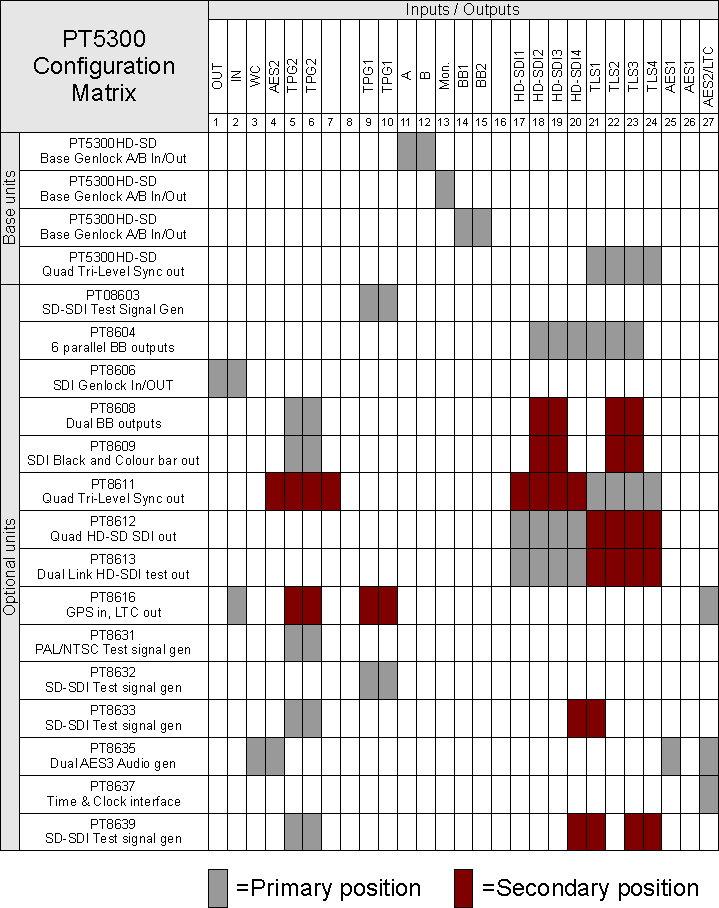
\includegraphics[width=0.8\textwidth]{fig/Config_matrix}

\caption{PT5300 Configurations }
\label{table:pt5300_config}

\end{figure}

\textbf{Note:} The function of some of the output/input connectors on the rear panel depends upon the functional modules/options included your generator and the functional configuration.

\begin{figure}[hbt]
\centering
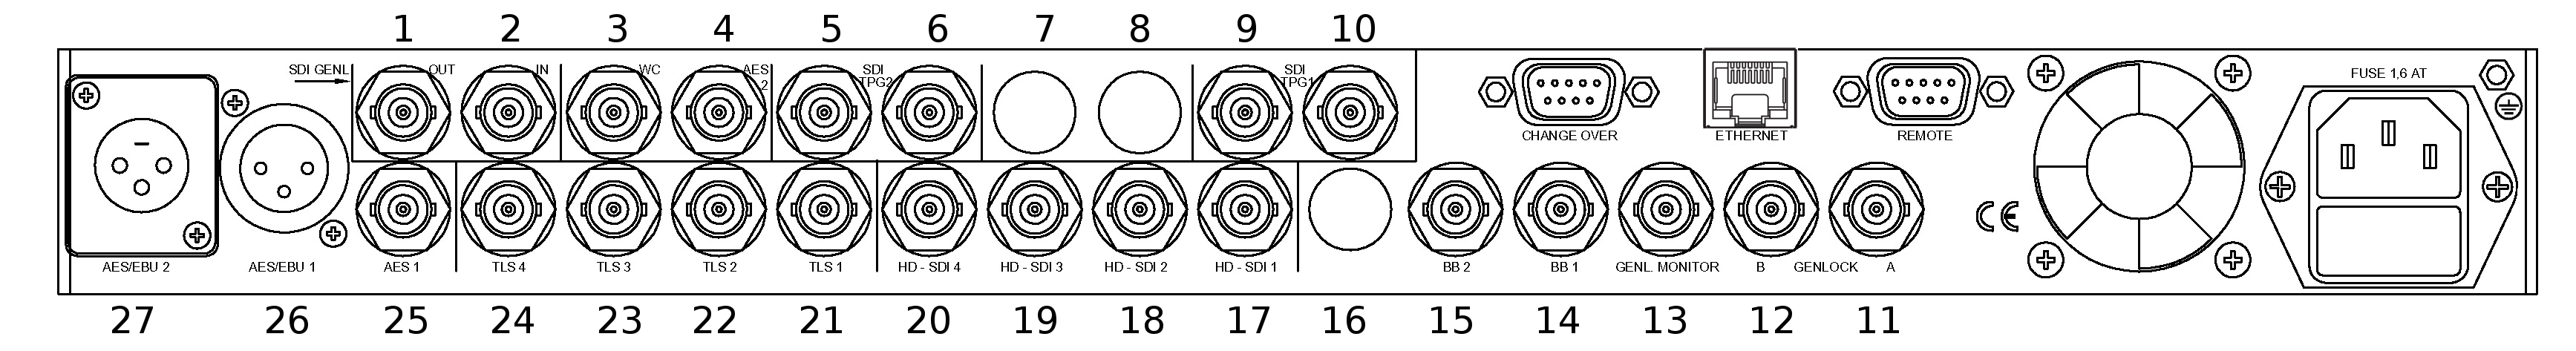
\includegraphics[width=\textwidth]{fig/PT5300_rear_config}
\caption{Rear Panel, Configuration}
\label{figure:pt5300_config}
\end{figure}

\subsection{Panel Operation}
The PT5300 HD-SD Varitime\TM Sync Generator may be equipped with several different optional modules. The menu system always reflects the modules installed. The operation of each of the modules is described below, although it is impossible for all the modules to be installed in one instrument at one time.

\subsubsection{Power Up}
A diagnostic routine is performed at power-on. After a normal start-up, the HD-SD Varitime\TM Sync Generator continues to the status display. If a failure is detected an error message is displayed.

\paragraph{Normal Start-up}
\display{HD-SD Sync. Gen.Power-up diagnose}{Selftest in progress \ldots}

This message is shown while the test is performed.

\textbf{After a successful test the following message is shown:}

\display{HD-SD Sync. Gen. Frame}{Version: 07.-03.0}

The instrument stops if errors are detected.
The diagnose may be continued if you press the \upbuttontext, \downbuttontext, \leftbuttontext, \rightbuttontext or \execute .
When the power-up diagnose program is finished, the instrument may be used, but excluding the erroneous function(s).

%\textit{Please see Appendix xxx for the list of errors detectable during power-up.}

\subsubsection{Status Displays}
If a preset was active at the previous power-down, this preset is automatically recalled and the preset status display is shown. The preset status display shows the number and name of the active preset.

\display{HD-SD Preset Status \leftbutton \downbutton \rightbutton}{PRESET (6):name of preset}
If genlock is activated in the preset and no genlock signal is identified, the status display will change to the genlock status display indicating UNLOCKED.

If no preset is active then genlock status display will be displayed.

Use the \leftbuttontext and \rightbuttontext buttons to select the status displays you want.

\textbf{Note:} The status displays for the various options are only available when the options are
installed.









\paragraph{Status:Preset}
\display{HD-SD Preset Status \leftbutton \downbutton \rightbutton}{NO PRESET ACTIVE}
\display{HD-SD Preset Status \leftbutton \downbutton \rightbutton}{PRESET (1):name of preset}

\paragraph{Status: Genlock}
\display{Genlock:A \leftbutton \downbutton \rightbutton}{Signal:PAL Burst Status: GENLOCKED}
\display{Genlock:Internal \leftbutton \downbutton \rightbutton}{Signal:-------Status:-------}

The genlock status display shows the input selected for genlock and the format of genlock selected. If the signal is NTSC or PAL the display will also indicate whether sync lock or burst lock is being used.

\textbf{Status: Analogue test pattern generator}

\display{Analog TPG1:PLUGE \leftbutton \downbutton \rightbutton}{System:PAL w/PAL ID +TEXT}

The status display for the analogue test pattern generator shows the signal output from each the generator and the system selected. If the text or time clock is inserted into the test pattern, then the presence is shown.

\textbf{Status: SDI test pattern generator}

\display{SDI-TPG1:PLUGE \leftbutton \downbutton \rightbutton}{System:525/59.94.+TEXT +AUDIO +EDH}

The status display for serial digital test pattern generator shows the signal output from each generator and the system selected. Also the status for text (and clock), embedded audio, and EDH inserted into test signals/pattern is shown.

\textbf{Status: SDI Basic generator}

\display{SDI-TSG3:WINDOW 15\% \leftbutton \downbutton \rightbutton}{System:525/59.94. +AUDIO +EDH}

The serial digital test signal generator status display shows the signal output from each of the Basic SDI generators and the system selected. Also the status for embedded audio and EDH is shown. No text or clock can be inserted.

\textbf{Status: AES/EBU Audio Generator}

\display{AES/EBU1:Stereo EBU 1kHz \leftbutton \downbutton \rightbutton}{Level:-9dBFS Timing:PAL}

The status display for the AES/EBU digital audio generator shows the output signal and level of the audio. The five NTSC phases or the PAL timing phase is also displayed.

\textbf{Status: DATE-TIME}

\display{DATE:05-02-02 TIME:14:05:05 ?? \leftbutton \downbutton \rightbutton}{REF: VITC Code STATUS: LOCKED}
This display shows the current status of date and time i.e. the information inserted into the video signal.

\textbf{Status: WARNING}

\display{HD-SD Error/Warning Status:?? \leftbutton \downbutton \rightbutton}{No error detected}
\display{HD-SD Error/Warning Status:?? \leftbutton \downbutton \rightbutton}{No active warning}
\display{HD-SD Error/Warning Status:?? \leftbutton \downbutton \rightbutton}{E(00n):mmmmmmmmmm}

The display shows the error/warnings status. The ``No error detector'' shows that no errors has been detected. The ``No active warning'' shows that no errors are present, but previously detected errors are stored in the ``Errorqueue''. In case of an error condition, the error number is shown in the display.
%\textit{Please refer to Appendix xxx for explanation of error messages}










\subsubsection{Menu Operation}
Pressing the \downbuttontext button in the status menu will cause the main menu to appear. This is the main route of access to all functions. If the control panel is locked, the padlock symbol will be flashing. Depending on which type of lock is used, it may have to be removed before some operations are allowed.

\textbf{To exit the STATUS menu, press the \downbuttontext button and move to the main menu:}

\display{HD-SD Sync Generator \leftbutton \updownbutton \rightbutton}{<BLACK-BURST> TRI-LEVEL HD-SDI \ldots}
\display{HD-SD Sync Generator \leftbutton \updownbutton \rightbutton}{<DL-SDI> ANALOG SDI-TSG4 \ldots}
\display{HD-SD Sync Generator \leftbutton \updownbutton \rightbutton}{<SDI-TPG1> SDI-TPG2 SDI-TPG5 \ldots}
\display{HD-SD Sync Generator \leftbutton \updownbutton \rightbutton}{<SDI-TPG2> AES-EBU <GENLOCK> \ldots}
\display{HD-SD Sync Generator \leftbutton \updownbutton \rightbutton}{LTC PRESET <CONFIG> \ldots}

\textbf{Note:} Not all of the above options can be installed at a time; maximum 2 HD-SD SDI boards and/or up to
3 TRI-LEVEL-SYNC and/or up 4 TSG's and/or up to 3 TPG's can be mounted at a time. For the
possible combinations, refer to figure \ref{figure:pt5300_config}. If one or more of the options is not installed, the keyword will be missing in the menu.

\textbf{Select one of the menus and go on to the next menu, e.g.:}

\display{MENU:BLACK-BURST, configure \leftbutton \updownbutton \rightbutton}{SUBMNU:<BB1> BB2}

The menus have basically the same structure and the same procedure is used with all the menus.
Select one of the items in the menu displayed
\begin{itemize}
\item Make a selection in the next menu below
\item Use the arrow buttons as indicated in the icon field
\item Select \save and press \execute to store the setting Select ESC and press \upbuttontext button to escape the menu or
\item Select the next menu level, i.e. 2NDMNU or
\item Confirm the selection by pressing \EXECUTE %(E is shown in the icon area)
\end{itemize}

\textbf{Note:} \save does not appear until a parameter is changed. Unintended changes are canceled by selecting ESC and returning to the level above.

\subsection{Detailed Description of Menus}






\subsubsection{Menu: BLACK-BURST generator}
This is the menu for setting the parameters for the analogue Black Burst outputs. The analogue Black Burst outputs are named BB1 and BB2 connector on the back of the instrument.

\textbf{Setting of the BLACK-BURST generator:}

\display{MENU:BLACK-BURST, configure \leftbutton \updownbutton \rightbutton}{SUBMNU:<BB1>BB2}

\begin{itemize}
\item Use the \leftbuttontext and \rightbuttontext buttons to select BB1
\item Then press \downbuttontext to enter the submenu for BB1
\end{itemize}

\display{SUBMNU:BLACK-BURST/BB1,select \leftbutton \updownbutton \rightbutton}{2NDMNU:<SYSTEM> TIMING ScH-PHASE}
The 2NDMNU allows changes to be made in the parameters for the BB1 output.

\textbf{To change form NTSC to PAL, select SYSTEM}

\display{2NDMNU:../BB1/SYSTEM, select \leftbutton \updownbutton \rightbutton}{SYSTEM:<PAL w/PAL ID> SAVE ESC}

\textbf{Operation:}

\begin{itemize}
\item Use the \upbuttontext and \downbuttontext buttons to find the system setting you want.
\item When the desired system appears in the display, move the cursor to \save and press \EXECUTE to change the system setting
\item If no change is desired, move the cursor to ESC and press \upbuttontext
\end{itemize}

\textit{Leaving the function takes you back to the BLACK-BURST/BB1 submenu.}

\textbf{Analogue Black Burst generator system options:}

\begin{itemize}
\item NTSC
\item PAL
\item PAL w/PAL ID
\end{itemize}

\textbf{Note:} If the PAL Field 1 pulse in Line 7 is inserted, it is independent of the Sc-H phase setting. If the Sc-H phase has been adjusted, the Line 7 pulse will identify the field as if the phase had not been changed from the nominal setting.
When the system ``PAL w/PAL ID'' is selected, a pulse indicating PAL Field 1 is included Line 7.

\textbf{Note:} When changing the system from PAL to NTSC you must check the timing adjustment: a valid PAL timing may NOT be valid in NTSC. If the timing is not valid in NTSC then it will be reset to +0,+0,+0.

\textbf{To change the delay/advance timing for the BB1 output, select TIME.}

\display{2NDMNU:../BB1/TIMING, edit delay \leftbutton \updownbutton \rightbutton}{V:<+1> H:+008 T: +00124.3 SAVE ESC}

\textbf{Operation:}

\begin{itemize}
\item Use the \leftbuttontext or \rightbuttontext buttons to select V, H, or T
\item Then use the \upbuttontext and \downbuttontext buttons to change the setting changes to the timing are instantaneous, i.e. any changes are reflected immediately in the output signal
\item When the desired setting appears in the display, move the cursor to \save and press \EXECUTE to change the setting
\end{itemize}

The timing can be adjusted by coarse or fine adjustment parameters. The coarsest adjustment is field (V) the finest is time (T), and line (H) is in between. The T value is in nanoseconds.
\begin{itemize}
\item The T value can be changed by using the \upbuttontext and \downbuttontext buttons to adjust the smallest step for the adjustment, but a faster method is to press \EXECUTE when the cursor is on the T value. This opens an editor in which each of the time digits can be changed using the \upbuttontext and \downbuttontext buttons
\item Positions are Selected by using the \leftbuttontext and \rightbuttontext buttons
\item To exit the editor press \EXECUTE
\item When the desired delay setting appears in the display, move the cursor to \save and press \EXECUTE
\item If no changes are desired, move the cursor to ESC and press \upbuttontext
\end{itemize}

\textit{Leaving the function takes you back to the BLACK-BURST/BB1 submenu.}

\textbf{To change the Sc-H phase of the BB1 output, select ScH-PHASE}

\display{2NDMNU:../BB1/SCH-PHASE, EDIT \leftbutton \updownbutton \rightbutton}{ScH-PHASE:<+5deg> SAVE ESC}
The default Sc-H phase for the BB outputs is 0 degrees. The value can be changed in steps of 1 degree.

\textbf{Operation:}

\begin{enumerate}
\item Use the \upbuttontext and \downbuttontext buttons to change the Sc-H phase. Change to the Sc-H phase is instant, i.e. any change made in the display is reflected immediately in the output signal
\item When the desired setting appears in the display, move the cursor to \save and press
\item EXECUTE
\item If no change is desired, move the cursor to ESC and press \upbuttontext
\end{enumerate}
\textit{Leaving the function takes you back to the BLACK-BURST/BB1 submenu.}








\subsubsection{Menu: TRI-LEVEL sync generator}
This is the menu for setting the parameters for the analogue TRI-LEVEL SYNC outputs.

The analogue TRI-LEVEL outputs are named TLS1, TLS2, TLS3, TLS4 when the units is
mounted in the primary position and TLS5, TLS6, TLS7, TLS8 when the units is mounted in the
additional / alternate position as mentioned in the table 6-1 on page 6-30

\textbf{Setting of the TRI-LEVEL SYNC generator:}

\display{MENU:TRI-LEVEL, configure \leftbutton \updownbutton \rightbutton}{SUBMNU:<TLS1> TLS2 TLS3 TLS4}

\begin{itemize}
\item Use the \leftbuttontext and \rightbuttontext buttons to select TLS1
\item Then press \downbuttontext to enter the submenu for TLS1
\end{itemize}

\display{SUBMNU:TRI-LEVEL/TLS1,select \leftbutton \updownbutton \rightbutton}{2NDMNU:<SYSTEM> TIMING}
The 2NDMNU allows changes to be made in the parameters for the TLS1 output.

\textbf{To change from one HD TRI-LEVEL format to another, select FORMAT}

\display{2NDMNU:../TLS1/SYSTEM, select \leftbutton \updownbutton \rightbutton}{SYSTEM:<HD 1080I/25> SAVE ESC}

\textbf{Operation:}

\begin{itemize}
\item Use the \upbuttontext and \downbuttontext buttons to find the format setting you want.
\item When the desired system appears in the display, move the cursor to \save and press \EXECUTE to change the format setting
\end{itemize}

\display{2NDMNU:../TLS1/SYTEM, select \leftbutton \rightbutton \execute}{SYSTEM:HD 1080I/25 <SAVE> ESC}

\begin{itemize}
\item If no change is desired, move the cursor to ESC and press \upbuttontext
\end{itemize}

\textit{Leaving the function takes you back to the TRI-LEVEL/TLS1 submenu.}

\textbf{Analogue TRI-LEVEL SYNC generator system options:}

\begin{itemize}
\setlength{\itemsep}{1pt}
\setlength{\parskip}{0pt}
\item 1080p/60
\item 1080p/59.94
\item 1080p/50
\item 1080p/30
\item 1080p/29.97
\item 1080p/25
\item 1080p/24
\item 1080p/23.96
\item 1080i/30
\item 1080i/29.97
\item 1080i/25
\item 720p/60
\item 720p/59.94
\item 720p/50
\item 720p/30
\item 720p/29.97
\item 720p/25
\item 720p/24
\item 720p/23.9
\end{itemize}

\textbf{Note:} When changing from one format to the other you must check the timing adjustment, as the timing in one format may NOT be valid in a different format. If the timing is not valid then it will be reset to +0,+0,+0.

\textbf{To change the delay/advance timing for the TLS1 output, select TIMING.}

\display{2NDMNU:../TLS1/TIMING, edit delay \leftbutton \updownbutton \rightbutton \execute}{F:<+1> H:+008 T: +00006.7 SAVE ESC}

\textbf{Operation:}

\begin{itemize}
\item Use the \leftbuttontext or \rightbuttontext buttons to select F, H, or T
\item Then use the \upbuttontext and \downbuttontext buttons to change the setting. Changes to the timing are instantaneous, i.e. any changes are reflected immediately in the output signal.
\item When the desired setting appears in the display, move the cursor to \save and press \EXECUTE to change the setting.
\end{itemize}

The timing can be adjusted by coarse or fine adjustment parameters. The coarsest adjustment is field (F) the finest is time (T), and line (H) is lines. The T value is in nanoseconds.

\begin{itemize}
\item The T value can be changed by using the \upbuttontext and \downbuttontext buttons to adjust the smallest step for the adjustment, but a faster method is to press \EXECUTE when the cursor is on the T value. This opens an editor in which each of the time digits can be changed using the \upbuttontext and \downbuttontext buttons.
\item Positions are Selected by using the \leftbuttontext and \rightbuttontext buttons.
\item To exit the editor press \EXECUTE
\item When the desired delay setting appears in the display, move the cursor to \save and press \EXECUTE
\item If no changes are desired, move the cursor to ESC and press \upbuttontext
\end{itemize}

\textit{Leaving the function takes you back to the TRI-LEVEL/TLS1 submenu.}








\subsubsection{Menu: GENLOCK}
This is the menu for setting the genlock parameters, which are the common reference for the individual timing of each generator.

It is always possible to genlock to analogue signals, while the PT 8606 SDI Digital Genlock option is necessary in order to genlock to digital video. The standard genlock inputs are designated A and B, and they can be either configured to signals terminated with 75 \ohm or configured as a high impedance loop-through.

The genlock function can be configured to different inputs and signals. Which signals are valid for each of the inputs depends on the setting in the Genlock menu.

\textbf{Select: GENLOCK}

\display{MENU : GENLOCK, select input \leftbutton \updownbutton \rightbutton}{<INTERNAL> SYS TIMING ESC}
\display{MENU : GENLOCK, select input \leftbutton \updownbutton \rightbutton}{<A PAL Burst> SYS TIMING OK ESC}

\textbf{Operation:}

\begin{itemize}
\item When an input has been configured to a specific type of genlock, this will be shown in the genlock select input menu
\item Use the \upbuttontext and \downbuttontext buttons to scroll through the different input options (with attached genlocked
types)
\item Then move the cursor to OK and press \EXECUTE button to change the selection (OK is only visible for other selections than the active)
\item If no change is desired, move the cursor to ESC and press \upbuttontext
\end{itemize}

\textit{Leaving the function takes you back to the GENLOCK menu.}

\textbf{The types of inputs available are:}

\begin{itemize}
\item A xxxxxx: Input A terminated 75 \ohm
\item B xxxxxx: Input B terminated 75 \ohm
\item A-B xxxxxx: Input A and B looped through, high impedance
\item Internal: The internal OCXO used as reference
\item SDI xxxxx: The optional PT 8606 SDI Digital Genlock module used for genlock input
\end{itemize}

Included with the selection is a description of the signal type used for the genlock. The xxxxxx reflects the genlock system selected in the SYStem submenu. For instance ``A-B PAL Burst'' indicates that loop-through A-B is configured for PAL burst lock.

\textbf{Note:} The ``UNLOCKED'' LED is ON when no correct genlock signal is found on the active genlock input.

\textbf{To change the genlock system for the input selected, select SYS in the GENLOCK menu.}

\display{SUBMNU:GENLOCK/SYSTEM, select \leftbutton \updownbutton \rightbutton}{SYSTEM:<PAL Burst> SAVE ESC}

\textbf{Operation:}

\begin{itemize}
\item Use the \upbuttontext and \downbuttontext buttons to select the system format of genlock for the input
\item  When the new format appears on the display, then move the cursor to \save and press \EXECUTE to change the signal format
\item  If no change is desired, move the cursor to ESC and press \upbuttontext 
\end{itemize}

\textit{Leaving the function takes you back to the GENLOCK menu.}

\textbf{Note:} Now the selected genlock system (A, B, Loop-through, Internal, or SDI) is configured. If the input for this system has not been activated, select OK in the GENLOCK menu and press \EXECUTE

Which signals are available to the different genlock inputs depends upon the type of genlock
edited.

\textbf{Genlock signals available for A, B, and A-B:}

\begin{itemize}
\setlength{\itemsep}{1pt}
\setlength{\parskip}{0pt}
\item PAL Burst
\item NTSC Burst
\item 625 Sync
\item 525 Sync
\item 4.43 MHz
\item 3.58 MHz
\item 5 MHz
\item 10 MHz
\end{itemize}

\textbf{Genlock signals available for SDI/GPS:}

\begin{itemize}
\item 525/59.94
\item 626/50
\end{itemize}

\textbf{Note:} No Genlock system nor Timing can be selected when Genlock Input is set to Internal or one of the continuous wave signals.

\textbf{To change the genlock timing for the input selected, select TIMING in the GENLOCK menu.}

\display{SUBMNU:GENLOCK/TIMING, edit delay \leftbutton \updownbutton \rightbutton}{V:<+0>H:+123 T:+00123.4 SAVE ESC}

\textbf{Operation:}

\begin{itemize}
\item Use the \leftbuttontext and \rightbuttontext buttons to select V, H, or T
\item Then use \upbuttontext or \downbuttontext buttons to select the value desired. Changes to the timing are instantaneous, i.e. any changes are reflected immediately in the output signal.
\end{itemize}

The timing can be adjusted by coarse or fine adjustment parameters. The coarsest adjustment is the Field (V), the finest is Time (T), and Line (H) is between. The T value is in nanoseconds. The timing resolution depends upon the type of signal used for genlock. 

\begin{itemize}
\item When the desired delay setting appears in the display, move the cursor to \save and press \EXECUTE
\item If no change is desired, move the cursor to ESC and press \upbuttontext 
\end{itemize}

\textit{Leaving the function takes you back to the GENLOCK menu}

\textbf{Note:} The genlock timing can only be changed when the genlock type is a signal containing line and field information. It is not possible to change timing when the reference is 5/10 MHz, Subcarrier frequency or internal.

\textbf{Note:} When changing genlock signal format, for instance, from PAL to NTSC, the timing parameters may become invalid: The timing parameter will then be reset to 0 for the input in question.









\subsubsection{Menu: GPS Genlock and LTC output}
This is the menu for setting the parameters for the GPS Genlock input and the LTC outputs.

\textbf{Select: GENLOCK}

\display{MENU : GENLOCK, select input \leftbutton \updownbutton \rightbutton}{<INTERNAL> SYS TIMING ESC}
\display{MENU : GENLOCK, select input \leftbutton \updownbutton \rightbutton}{<GPS 625/50> SYS TIMING OK ESC}

\textbf{Operation:}

\begin{itemize}
\item When an input has been configured to a specific type of genlock, this will be shown in the genlock select input menu
\item Use the \upbuttontext and \downbuttontext buttons to scroll through the different input options (with attached genlocked types)
\item Then move the cursor to OK and press \EXECUTE button to change the selection (OK is only visible for other selections than the active)
\item If no change is desired, move the cursor to ESC and press \upbuttontext Leaving the function takes you back to the GENLOCK menu.
\end{itemize}

\textit{Leaving the function takes you back to the GENLOCK menu.}

The LTC outputs are named LTC A and LTC B. LTC A and LTC B are output to both BNC connectors at the same time where on the XLR connector it is one at the time.

\textbf{Settings of the LTC generator:}

\display{SUBMNU: LTC, select 13:55:09 \leftbutton \updownbutton \rightbutton}{LTC A <OFFSET> FORMAT TIME SYNC ESC}

\begin{itemize}
\item Use the \upbuttontext and \downbuttontext buttons to switch between LTC A or B set-up, when marked as shown above. Notice, that switching between LTC A and B, only determines which generator to be setup, and does not yet alter the outputs.
\item Select the parameter, you wish to change, then press \downbuttontext to enter the parameter submenu for the selected LTC generator.
\end{itemize}

\textbf{To set offset, select OFFSET:}

\display{2NDMNU: ../LTC A/OFFSET, edit delay \leftbutton \updownbutton \rightbutton}{OFFSET: <+0000100000.0>ns OK ESC}

Each LTC generator can be individually timed, relative to absolute (GPS) time. The offset can be in the range of $\pm$500 ms, in steps of 6.7 ns.

\textbf{Operation:}

\begin{itemize}
\item Use the \upbuttontext and \downbuttontext buttons to increase/decrease delay. Pressing OK will apply the delay.
\item For faster adjustment, you can go into coarse mode. By pressing the \execute button, you can edit the individual digits. Select a digit by pressing 3 and 4, and edit the offset, by pressing \updownbuttontext. Notice, that the lowest digit cannot be selected. This is because the step-size is greater than what this digit represents.
\item When done, move the cursor to OK and \EXECUTE or move to ESC and press \upbuttontext to cancel. 
\end{itemize}
\textit{Leaving the function takes you back to the LTC submenu.}

\textbf{To change between formats, select FORMAT}

\display{2NDMNU: ../LTC A/FORMAT, select \leftbutton \updownbutton \rightbutton}{FORMAT: <25.00 FPS> SYNCMODE OK ESC}

\textbf{Operation:}

\begin{itemize}
\item Use the \upbuttontext and \downbuttontext buttons to find the system setting you want.
\item When the desired system appears in the display, press OK to confirm. Otherwise move the cursor to ESC and press \upbuttontext to cancel.
\end{itemize}

\textit{Leaving the function takes you back to the LTC submenu.}

\textbf{LTC options:}

\begin{itemize}
\setlength{\itemsep}{1pt}
\setlength{\parskip}{0pt}
\item 24 FPS
\item 25 FPS
\item 29.97 FPS Non-dropframe (in menu $<$29.97 NOND$>$)
\item 29.97 FPS Dropframe
\item 30 FPS
\end{itemize}

\textbf{Note:} When selecting 29.97 FPS modes, go to the main LTC menu, and select $<$SYNC$>$ to reset the frame-counter.

\textbf{To change how the 29.97 FPS LTC re-sync the frame-counter, select SYNCMODE}

\display{2NDMNU: ../LTC A/SYNCMODE, edit \leftbutton \updownbutton \rightbutton}{SYNCMODE:<AUTO> TIME: 00:00 OK ESC}

When running at 29.97 FPS, the frame counter does not match real-time. One second at 29.97 FPS are a bit longer than a real-time second. Therefore, the LTC time lags behind realtime after a while. To prevent this, the LTC generator can re-sync the frame-counter. The LTC generator can do this in three modes: NONE, CONFIRM mode and AUTO mode. When NONE is selected, the frame-counter never resets (you can reset the frame counter manually from the LTC main menu). In CONFIRM mode, the PT5300 will ask for confirmation at the time specified in the SYNCMODE menu. In AUTO mode, the frame counter re-syncs automatically, at the time specified in the SYNCMODE menu.

\textbf{Operation:}

\begin{itemize}
\item Use the \leftbuttontext and \rightbuttontext buttons to select either mode, hours or minutes.
\item Use the \upbuttontext and \downbuttontext buttons to find the mode you want.
\item Use the \upbuttontext and \downbuttontext buttons to specify, at which time the re-sync shall occur.
\item When the desired system appears in the display, press OK to confirm. Otherwise move the cursor to ESC and press \upbuttontext to cancel.
\end{itemize}

\textit{Leaving the function takes you back to the LTC submenu.}

\textbf{To change time and date settings, select TIME}

\display{2NDMNU: ../LTC A/TIME, select \leftbutton \updownbutton \rightbutton}{2NDMNU: <TIMEZONE> DAYLIGHT ESC}

In the TIME menu, the clock and date can be setup, as well as daylight saving parameters.

\textbf{Operation:}

\begin{itemize}
\item Use the \leftbuttontext and \rightbuttontext buttons to select the time setting you want alter, then press \downbuttontext
\item TIMEZONE and DAYLIGHT will open a new menu.
\end{itemize}

\textit{Leaving the function takes you back to the LTC submenu.}

\textbf{To change time zone, select TIMEZONE}

\display{2NDMNU: ../LTC A/TIMEZONE, edit \leftbutton \updownbutton \rightbutton}{TIMEZONE: +01:00 OK ESC}

In the TIMEZONE menu, you can set the time zone, by offsetting the UTC time in steps of 30 minutes.

\textbf{Operation:}

\begin{itemize}
\item Use the \leftbuttontext and \rightbuttontext buttons to select either hours or minutes.
\item Use the \upbuttontext and \downbuttontext buttons to set the desired offset.
\item When the desired UTC offset appears in the display, move the cursor to OK and press \EXECUTE
\end{itemize}

\textit{Leaving the function takes you back to the TIME submenu.}

\textbf{To change daylight saving options, select DAYLIGHT}

\display{2NDMNU: ../LTC A/DAYLIGHT, select \leftbutton \updownbutton \rightbutton}{MODE:<AUTO>DST: on START END OK ESC}

In the DAYLIGHT menu, the daylight saving settings are made. There are three different modes, to choose from. AUTO mode switches to, and back from daylight saving time automatically. This means the time advances one hour, at the chosen start date, and resets at the end date. The PT5300 will notice you of this change. In CONFIRM mode, the PT5300 does NOT change the time automatically, but will instead notice you and wait for confirmation to switch time. In OFF mode, no daylight saving changes will be made. You can also immediately change the state, by setting DST (daylight saving time) on or off in the menu.

\textbf{Operation:}

\begin{itemize}
\item Use the \leftbuttontext and \rightbuttontext buttons to select desired parameter.
\item Use the \upbuttontext and \downbuttontext buttons to switch between modes, when marked.
\item Use the \upbuttontext and \downbuttontext buttons to switch daylight saving on/off, when marked.
\item Use the \downbuttontext button on START or END, to setup daylight saving start and end date.
\item Press \EXECUTE on OK to confirm settings
\end{itemize}

\textit{Leaving the function takes you back to the TIME submenu.}

\textbf{To change daylight savings start or end date, select START or END}

\display{3RDMNU:../LTC A/DAYLIGHT/START, edit \leftbutton \updownbutton \rightbutton}{START DATE:<03>29 HOUR: 02 OK ESC}

You can set month, day and hour for when the switching should occur.

\textbf{Operation:}

\begin{itemize}
\item Use the \leftbuttontext and \rightbuttontext buttons to select month, day or hour.
\item Use the \upbuttontext and \downbuttontext buttons to set the desired month/date/time.
\item When the desired month/date/time appears in the display, move the cursor to OK and press \EXECUTE to store or press \upbuttontext on ESC to cancel.
\end{itemize}

\textit{Leaving the function takes you back to the DAYLIGHT submenu.}



%-------------------------------------------------------ETHERNET START----------------------------------------------------
\newpage
\subsubsection{Menu: NETWORK}
\label{cha:NETWORK}
This is the menu for setting the parameters for the PT8643 Ethernet module.

\textbf{Ethernet settings:}

%\display{SUBMNU: NETWORK, select \leftbutton \updownbutton \rightbutton}{<ETHERNET> CONFIG ESC}
\display{SUBMNU: NETWORK, select \leftbutton \downbutton \rightbutton}{<ETHERNET> CONFIG ESC}

\begin{itemize}
\item Use the \leftbuttontext and \rightbuttontext buttons to select ETHERNET.
\item Then press \downbuttontext to enter the ETHERNET submenu.
\end{itemize}

%\display{2NDMNU: ../NETWORK/ETHERNET \leftbutton \downbutton \rightbutton}{<DHCP> IP ADDR  SUBNET MASK  GATEWAY}
\display{2NDMNU: ../NETWORK/ETHERNET \leftbutton \downbutton \rightbutton}{<DHCP> IP ADDR  SUBNET MASK  GATEWAY}
\textbf{The following options is available in the ETHERNET menu:}

\begin{itemize}
\item DHCP - Enable or disable the DHCP client.
\item IP ADDR - Manually configure the IP address.
\item SUBNET MASK - Manually configure the subnet mask.
\item GATEWAY - Manually configure the gateway.
\item MAC ADDR - View the PT8643 MAC address.
\item NETFINDER - View the NetFinder name.
\item ESC - Return to the NETWORK menu.
\end{itemize}

The DHCP client is enabled as default. When DHCP is enabled the menus IP ADDR, SUBNET MASK and GATEWAY is read only.\\

\textit{Leaving the function using ESC takes you back to the NETWORK menu.}\\

\textbf{Disable the DHCP client (Set a static IP address):}
%\display{2NDMNU: ../NETWORK/ETHERNET \leftbutton \rightbutton \ebutton}{DHCP: <On> Off ESC}
\display{2NDMNU: ../NETWORK/ETHERNET \leftbutton \rightbutton \ebutton}{DHCP: <On> Off ESC}

\textbf{Operation:}

\begin{itemize}
\item In the ETHERNET submenu use the \leftbuttontext and \rightbuttontext buttons to select DHCP and press \EXECUTE to enter the DHCP submenu.
\item Use the \leftbuttontext and \rightbuttontext buttons to select OFF and press \EXECUTE to disable DHCP.
	\begin{itemize}
		\item When selecting OFF you will automatically enter the IP ADDR submenu.
		\item When selecting ON you will automatically return to the ETHERNET submenu.
	\end{itemize}
\item If no change is desired, move the cursor to ESC and press \upbuttontext.\\ \textit{Leaving the function takes you back to the ETHERNET submenu.}
\end{itemize}

\newpage
\textbf{IP Address configuration:}
%\display{3RDMNU: ../IP ADDR, modify \leftbutton \rightbutton \ebutton}{000.000.000.001 OK <ESC>}
\display{3RDMNU: ../IP ADDR, modify \leftbutton \rightbutton \ebutton}{000.000.000.001 OK <ESC>}

\begin{itemize}
\item If not already in the IP ADDR submenu use the \leftbuttontext and \rightbuttontext buttons in the ETHERNET submenu to select IP ADDR and press \EXECUTE.
\item Use the \leftbuttontext and \rightbuttontext buttons to move the cursor between the fields.
\item Use the \upbuttontext and \downbuttontext buttons to change the IP address.
\item When the desired IP address has been entered, move the cursor to OK and press \EXECUTE to save the changes.
\item If no change is desired, move the cursor to ESC and press \upbuttontext.\\ \textit{Leaving the function takes you back to the ETHERNET submenu.}
\end{itemize}

\textbf{Subnet mask and gateway configuration:}\\

The subnet mask and gateway is configured the same way as the IP address using the SUBNET MASK and GATEWAY menus.\\

\textbf{View MAC address:}
%\display{2NDMNU: ../NETWORK/ETHERNET \leftbutton \updownbutton \rightbutton \ebutton}{MAC ADDR: 00:0b:3c:24:ae:5c <ESC>}
\display{2NDMNU: ../NETWORK/ETHERNET \leftbutton \updownbutton \rightbutton \ebutton}{MAC ADDR: 00:0b:3c:24:ae:5c <ESC>}
\textbf{Operation:}

\begin{itemize}
\item In the ETHERNET submenu use the \leftbuttontext and \rightbuttontext buttons to select MAC ADDR. Then press the \downbuttontext button to enter the MAC address submenu.
\item The MAC address submenu will show the MAC (Media Access Control) address assigned to the PT8643. This address is globally unique and the first part of the address will always start with 00:0b:3c.
\item Use the \updownbuttontext to exit the menu.\\ \textit{Leaving the function takes you back to the ETHERNET submenu.}
\end{itemize}

\textbf{View NetFinder name:}\\
%\display{2NDMNU: ../NETWORK/ETHERNET \leftbutton \updownbutton \rightbutton \ebutton}{Unnamed. <ESC>}
\display{2NDMNU: ../NETWORK/ETHERNET \leftbutton \updownbutton \rightbutton \ebutton}{Unnamed. <ESC>}
\textbf{Operation:}

\begin{itemize}
\item In the ETHERNET sub menu use the \leftbuttontext and \rightbuttontext buttons to select NETFINDER and press the \downbuttontext button to enter the NetFinder submenu.
\begin{itemize}
	\item The NetFinder submenu will show the user assigned name of the PT5300.
	\item The NetFinder name can be up to 32 characters long.
	\item The Netfinder name is on the network used by the PC software DK-5300 to easily distinguish multiple PT5300 from each other.
	\item The NetFinder name can not be changed locally. It must be changed from the PC Software DK-5300.
	\item The NetFinder name is not visible if an Ethernet link has not been established.
	\item Please see section \ref{cha:DK5300} for further information about the NetFinder protocol and DK-5300.
\end{itemize}
\item Use the \updownbutton buttons to exit the menu.\\ \textit{Leaving the function takes you back to the ETHERNET submenu.}
\end{itemize}

\textbf{Network configuration:}

\begin{itemize}
\item In the NETWORK menu use the \leftbuttontext and \rightbuttontext buttons to select CONFIG.\\
\display{SUBMNU: NETWORK, select \leftbutton \downbutton \rightbutton}{ ETHERNET <CONFIG> ESC}
\item Then press \downbuttontext button to enter the CONFIG submenu.
\end{itemize}


\display{2NDMNU: ../NETWORK/CONFIG \leftbutton \updownbutton \rightbutton}{<TELNET>  PORT  RESET PASSWORD  ESC}

\textbf{The following options is available in the CONFIG menu:}
\begin{itemize}
\item TELNET - Enable or disable the Telnet Server.
\item PORT - View the Telnet port number.
\item RESET PASSWORD - Reset the network user name and password to default.
\item ESC - Return to the NETWORK menu.
\end{itemize}

\textit{Leaving the function using ESC takes you back to the NETWORK menu.}\\

The Telnet server is used for remote control of the PT5300 over the network.\\

The Telnet Server is enabled as default.\\

\textbf{Disable the Telnet server:}
\display{2NDMNU: ../NETWORK/CONFIG \leftbutton \rightbutton \ebutton}{TELNET: <On> Off ESC}

\textbf{Operation:}

\begin{itemize}
\item Use the \leftbuttontext and \rightbuttontext buttons to select TELNET and press the \downbuttontext button to enter the TELNET submenu.
\item Use the \leftbuttontext and \rightbuttontext buttons to select OFF and press \EXECUTE to disable the Telnet server.
	\begin{itemize}
		\item The Telnet Enable/Disable function can only be controlled locally.
	\end{itemize}
\item If no change is desired, move the cursor to ESC and press \upbuttontext.\\ \textit{Leaving the function takes you back to the CONFIG submenu.}
\end{itemize}

\textbf{View the Telnet port number:}
\display{2NDMNU: ../NETWORK/CONFIG \leftbutton \rightbutton \ebutton}{PORT: 23 <ESC>}

\textbf{Operation:}

\begin{itemize}
\item In the CONFIG submenu use the \leftbuttontext and \rightbuttontext buttons to select PORT and press the \downbuttontext button to enter the PORT submenu.
	\begin{itemize}
		\item The Telnet server is as default configured to listen on port 23.
		\item The Telnet port number can not be changed locally. It must be changed from the PC Software DK-5300.
		\item Please see section \ref{cha:DK5300} for further information about the NetFinder protocol and DK-5300.
	\end{itemize}
\item If no change is desired, move the cursor to ESC and press \upbuttontext.\\ \textit{Leaving the function takes you back to the CONFIG submenu.}
\end{itemize}

\textbf{Reset the user name and password to default:}
\display{2NDMNU: ../NETWORK/CONFIG \leftbutton \rightbutton \ebutton}{RESET PASSWORD  <OK> ESC}

\textbf{Operation:}

\begin{itemize}
\item In the CONFIG submenu use the \leftbuttontext and \rightbuttontext buttons to select RESET PASSWORD and press the \downbuttontext button to enter the RESET PASSWORD submenu.
\item To reset the user name and password to default use the \leftbuttontext and \rightbuttontext buttons to select OK and press \EXECUTE.
	\begin{itemize}
		\item The user name will be reset to \textbf{\DefaultUser}  and the password will be reset to \textbf{\DefaultPass}  .
		\item The user name and password is case sensitive.
		\item The user name and password can each have a length of 16 characters.
		\item The user name and password can be configured from the PC software DK-5300.
		\item Please see section \ref{cha:DK5300} for further information about the NetFinder protocol and DK-5300.
	\end{itemize}
\item If no change is desired, move the cursor to ESC and press \upbuttontext.\\ \textit{Leaving the function takes you back to the CONFIG submenu.}
\end{itemize}

\PasswordWarning
%--------------------------------------------------------ETHERNET END-----------------------------------------------------




\subsubsection{Menu: PRESET}
\display{MENU:PRESET, select function \leftbutton \updownbutton \rightbutton}{SUBMNU:<RECALL> STORE NAME \ldots}

\textbf{To recall the Preset, select RECALL}

\display{SUBMNU:PRESET/RECALL select \leftbutton \updownbutton \rightbutton}{RECALL (PRESET 1) OK ESC}

\textbf{Operation:}

\begin{itemize}
\item Use the \upbuttontext and \downbuttontext buttons to select preset.
\item When the desired preset appears in the display, move the cursor to OK and press \EXECUTE. If no change is desired, move the cursor to ESC and press \upbuttontext
\end{itemize}

\textit{Leaving the function takes you back to the PRESET menu, or if a preset is recalled the Preset Status display will be activated}

Whenever a recall is activated, it will apply to the generator until a value in the operation is altered. If a preset has been canceled, the only way to activate it again is to recall the preset. 

If a preset is active when you enter the submenu, the submenu will show the selected preset; otherwise Preset 1 will be selected.

\textbf{When using the PRESET button:}

\begin{itemize}
\item If a preset is active, pressing the PRESET button will bring up the recall [number], the number in brackets being the preset currently active
\item If no preset is active, pressing the PRESET button will bring up "Recall [1]"
\item The PRESET button, if you press it repeatedly, will act like the up button, i.e. the next preset is selected
\end{itemize}

\textbf{To store the Preset, select STORE}

\display{SUBMNU:PRESET/STORE, select \leftbutton \updownbutton \rightbutton}{STORE1:<PRESET1> OK ESC}

\textbf{Operation:}

\begin{itemize}
\item Use the \upbuttontext and \downbuttontext to select the preset no. to store
\item When the desired preset appears in the display, move the cursor to OK and press \EXECUTE
\item If no change is desired, move the cursor to ESC and press \upbuttontext leaving the function takes you back to the PRESET menu.
\end{itemize}

\textbf{To edit the Preset name, select NAME}

\display{2NDMNU:PRESET/NAME, edit name \leftbutton \updownbutton \rightbutton \execute}{NAME1:<PRESET1> SAVE ESC}

\textbf{Operation:}

\begin{itemize}
\item Use the \upbuttontext and \downbuttontext buttons to select the preset to be named
\item When the desired preset appears in the display press the button \EXECUTE to open the text editor
\item Use \leftbuttontext button to delete characters while backspacing
\item Scroll through the characters with the \leftbuttontext and \rightbuttontext buttons. The characters being edited will flash during the editing process.
\item When the desired characters appears, use the \leftbuttontext button to move to the next character to be inserted.
\item To exit the editor press \EXECUTE
\item To store the programmed line and status, move the cursor to \save and press \EXECUTE
\item  If no change is desired, move the cursor to ESC and press \upbuttontext . Leaving the function takes you back to the PRESET menu.
\end{itemize}









\subsubsection{Menu: CONFIG}
This is the menu for setting parameters not related to the specific output signals.

\display{MENU:CONFIG, select function \leftbutton \updownbutton \rightbutton}{SUBMNU:<DATE-TIME> LOCK AUTO-ESC \ldots}
\display{MENU:CONFIG, select function \leftbutton \updownbutton \rightbutton}{SUBMNU:<LCD-CONTRAST> DOWNLOAD \ldots}
\display{MENU:CONFIG, select function \leftbutton \updownbutton \rightbutton}{SUBMNU:<RS232 > DIAGNOSE \ldots}

\begin{itemize}
\item Use the \leftbuttontext and \rightbuttontext buttons to select the parameter to be change 
\item Then press the \downbuttontext button to enter the submenu
\end{itemize}

\textbf{Note:} The menu-item ``DATE-TIME'' is only shown when the PT 8637 Time Clock Interface is mounted.

\textbf{To change the date and time, select DATE-TIME}

The menu is only present with the PT 8637 Time Clock Module mounted.

\display{SUBMNU:CONFIG/DATE-TIME, configure \leftbutton \updownbutton \rightbutton}{2NDMNU:<DATE> TIME REFERENCE \ldots}
\display{SUBMNU:CONFIG/DATE-TIME, configure \leftbutton \updownbutton \rightbutton}{2NDMNU:<OFFSET> \ldots}

\begin{itemize}
\item Use the \leftbuttontext and \rightbuttontext buttons to select the parameter to be change
\item Then press the \downbuttontext button to enter the 2nd menu
\end{itemize}

\textbf{To change the date, select DATE}

\display{2NDMNU:../DATE-TIME/DATE, modify \leftbutton \updownbutton \rightbutton}{DATE:<YY-MM-DD> 98-05-01 \ldots}

\textbf{Operation:}

\begin{itemize}
\item Use the \leftbuttontext and \rightbuttontext buttons to select the parameter to change.
\item Use the \upbuttontext and \rightbuttontext buttons to change the date format.
\item When the desired format appears in the display and /or the date has been set, move the cursor to \save and press \EXECUTE
\item Then move the cursor to ``DATE FIELD'' and press \EXECUTE to open an editor in which each digit can be set separately using the \upbuttontext and \downbuttontext buttons. Using the \leftbuttontext and \rightbuttontext buttons to select digit.
\item To exit the editor press \EXECUTE. If the edited date is invalid, it will be reset to actual date.
\item If no change is desired, move the cursor to ESC and press \EXECUTE
\end{itemize}

\textit{ Leaving the function takes you back to the CONFIG/DATE-TIME submenu}

First field selects between different date formats:

\begin{itemize}
\item YY-MM-DD
\item DD-MM-YY
\item MM-DD-YY
\end{itemize}

The second field is showing the actual date.

\textbf{To change the time, select TIME}

\display{2NDMNU:../DATE-TIME/TIME, modify \leftbutton \updownbutton \rightbutton}{TIME:<24h> 14:19:53 \ldots}

\textbf{Operation:}

\begin{itemize}
\item Use the \leftbuttontext and \rightbuttontext buttons to select the parameter to change.
\item Use the \upbuttontext and \downbuttontext buttons to change the time format.
\item When the desired format appears in the display and /or the time has been set, move the cursor to \save and press \EXECUTE. If the edited time is invalid, it will be reset to actual time.
\item Then move the cursor to ``TIME FIELD'' and press \EXECUTE to open an editor in which each digit can be set separately using the \upbuttontext and \downbuttontext buttons. Using the \leftbuttontext and \rightbuttontext buttons to select digit.
\item To exit the editor press \EXECUTE
\item When the time has been set, move the cursor to \save and press \EXECUTE
\item If no change is desired, move the cursor to ESC and press \EXECUTE
\end{itemize}

\textit{Leaving the function takes you back to the CONFIG/DATE-TIME submenu}

First field selects between different time formats:
\begin{itemize}
\item 24 hours
\item 12 hours
\end{itemize}

The second field is showing the actual time.

\textbf{To change the reference for Date and Time, select REFERENCE}

\display{2NDMNU:../DATE-TIME/REFERENCE \leftbutton \updownbutton \rightbutton}{REFERENCE:<LTC Input> \ldots}

\textbf{Operation:}

\begin{itemize}
\item Use the \upbuttontext and \downbuttontext buttons to change the parameter
\item When the desired reference appears in the display, move the cursor to \save and press \EXECUTE
\item If no change is desired, move the cursor to ESC and press \upbuttontext
\end{itemize}

\textit{Leaving the function takes you back to the CONFIG/DATE-TIME submenu.}

\textbf{Reference options:}

\begin{itemize}
\item ``LTC-input'' via XLR connector ``TIME CODE''.
\item ``1 Hz Reference'' via XLR connector.
\item ``VITC on genlock'' time information in genlock signal.
\item ``Video Field Freq'', Clock tick rate derived from master oscillator locked to the genlock input.
\end{itemize}

\textbf{To change the time offset for Date and Time, select OFFSET}

\display{2NDMNU:../DATE-TIME/OFFSET \leftbutton \updownbutton \rightbutton}{OFFSET:<10.0> \ldots}

\textbf{Operation:}

\begin{itemize}
\item Use the \upbuttontext and \downbuttontext buttons to change the offset time. Step size is 0.1 second
\item When the desired offset has been achieved, move the cursor to \save and press \EXECUTE
\item If no change is desired, move the cursor to ESC and press \upbuttontext
\end{itemize}

\textit{Leaving the function takes you back to the CONFIG/DATE-TIME submenu.}

\textbf{To change the lockout function for the keyboard, select LOCK}

\display{MENU: CONFIG/LOCK, Normal (Off) \leftbutton \updownbutton \rightbutton}{LOCK:<Normal> On SAVE ESC}
\display{MENU: CONFIG/LOCK, Normal (On ) \leftbutton \updownbutton \rightbutton}{LOCK:<Normal> Off SAVE ESC}

\textbf{Description:}
The lock function enables/disables different levels of keyboard operation lockout. 

Select NORMAL for partial keyboard lockout. In this mode, the \textbf{C.BAR, M.BURST, WINDOW/FLAT, SPECIAL, LINEARITY, PATTERN, PRESET,} and the \textbf{OUTPUT} buttons are enabled

The \textbf{PRESET} button operates as a shortcut key to recall presets; stored presets can be recalled but not changed.

The \textbf{OUTPUT} button operates as a short-cut key to the signal generators. The button toggles between the all test signal generators, if more than one is installed.

\textbf{Note:} If the setup has no test signal generator, the \textbf{OUTPUT} button has no function.

\textbf{Note:} A padlock will appear in the top right corner of the display of a locked function.

\display{SUBMNU:CONFIG/LOCK, Panel(Off) \leftbutton \updownbutton \rightbutton}{LOCK:<Panel> On SAVE ESC}
\display{SUBMNU:CONFIG/LOCK, Panel(On) \leftbutton \updownbutton \rightbutton}{LOCK:<Panel> Off SAVE ESC}

Select PANEL for maximal lockout. In this mode no operations are possible, except unlock.

\display{SUBMNU:CONFIG/LOCK, Download(On) \leftbutton \updownbutton \rightbutton}{LOCK:<Download> Off SAVE ESC}
\display{SUBMNU:CONFIG/LOCK, Download(Off) \leftbutton \updownbutton \rightbutton}{LOCK:<Download> On SAVE ESC}

To lock the download function, select DOWNLOAD

\display{SUBMNU:CONFIG/LOCK, Date-Time(On) \leftbutton \updownbutton \rightbutton}{LOCK:<Date-Time> Off SAVE ESC}
\display{SUBMNU:CONFIG/LOCK, Date-Time(Off) \leftbutton \updownbutton \rightbutton}{LOCK:<Date-Time> On SAVE ESC}

To lock the fate and time setting function, select DATE-TIME. This function is only available when PT8637 Time Clock Interface is mounted.

\display{SUBMNU:CONFIG/LOCK, Diagnose(Off) \leftbutton \updownbutton \rightbutton}{LOCK:<Diagnose> On SAVE ESC}
\display{SUBMNU:CONFIG/LOCK, Diagnose(On) \leftbutton \updownbutton \rightbutton}{LOCK:<Diagnose) Off SAVE ESC}

To lock the diagnostic program, select DIAGN0SE. The diagnostic program tests the internal functioning of the generator.

\textbf{Note:} The diagnostic program is non-destructive of generator setting. When the diagnostic program is running, the output signals may be momentarily distorted.

\textbf{To change the menu auto escape function, select AUTO-ESCAPE.}

\display{SUBMNU:CONFIG/AUTO-ESC, select \leftbutton \updownbutton \rightbutton}{AUTO RETURN TO STATUS:<Off> SAVE ESC}

\textbf{Auto ESC options:}

\begin{itemize}
\item Off
\item On
\end{itemize}

When the instrument is left in a menu mode, the AUTO ESCAPE function returns the instrument
to the last active status display if no key has been activated for 60 seconds.

If the auto escape is disabled, the menu mode will remain active.

\textbf{To change the contrast level of the display, select LCD-CONTRAST.}

\display{SUBMNU:CONFIG/LCD-CONTRAST, set \leftbutton \updownbutton \rightbutton}{<xxxx          > ESC}

Use the \upbuttontext and \downbuttontext keys to change the contrast level of the display

\textbf{To copy the instrument settings from one generator to another, select DOWNLOAD.}

The DOWNLOAD function is used when two generators are directly connected by an RS232 interface cable. The cable must be connected to the remote connector on both generators. 

The generator to be programmed functions as the master in the procedure. The source generator operates undisturbed during the download procedure.

\display{SUBMNU:CONFIG/DOWNLOAD, select \leftbutton \updownbutton \rightbutton}{DOWNLOAD:<Preset\#1> OK ESC}

When the desired download selection is displayed select OK and press \EXECUTE

\textbf{SPG download options:}

\begin{itemize}
\setlength{\itemsep}{1pt}
\setlength{\parskip}{0pt}
\item Preset \#1
\item Preset \#2
\item Preset \#3
\item Preset \#4
\item Preset \#5
\item Preset \#6
\item All Presets
\end{itemize}

Select PRESET \#N to download the programming for a specific preset. The programming will be copied to the same preset number in the target generator as is used in the source generator. Select ALL PRESETS to copy all six preset.

\textbf{Note:} Whenever the DOWNLOAD functions are used, either the SPG used must be identical or the modules referred to in the presets must be available at the same positions in both generators.

\begin{itemize}
\item To abort the download, press \upbuttontext
\item  The instrument returns to normal operation after completed downloading. If the complete instrument setting has been copied, the instrument will operate according to this setting
\end{itemize}

\begin{center}
\fbox{
\parbox{0.95\textwidth}{
\textbf{CAUTION:} Selecting ESC during the downloading process will not reset to the values in use before the downloading process was started. ESC will reset the programming of the selected preset number or the entire instrument to its original factory programming!
}}
\end{center}

%\textbf{To configure the RS232 remote communication, select RS232.}
\textbf{To view the RS232 remote communication settings, select RS232.}

\display{SUBMNU:CONFIG/RS232, select \leftbutton \updownbutton \rightbutton}{2NDMNU:<BAUD-RATE> DATA-BIT PARITY \ldots}
\display{SUBMNU:CONFIG/RS232, select \leftbutton \updownbutton \rightbutton}{2NDMNU:<HANDSHAKE> \ldots}

\begin{itemize}
\item The RS232 settings can not be changed.
\item Use the \leftbuttontext and \rightbuttontext buttons to select the parameter to be accessed.
\item Then press the \downbuttontext button to enter the submenu for parameter setting in the RS232 interface.
\end{itemize}

%\begin{itemize}
%\item Use the \leftbuttontext and \rightbuttontext buttons to select the parameter to be changed
%\item Then press the \downbuttontext button to enter the submenu for parameter setting in the RS232 interface
%\end{itemize}
%
%\textbf{To set the RS232 interface speed, select BAUD-RATE}
%
%\display{2NDMNU:../RS232/BAUD-RATE, select \leftbutton \updownbutton \rightbutton}{BAUD-RATE:<300> SAVE ESC}
%
%\textbf{Operation:}
%
%\begin{itemize}
%\item Use the \upbuttontext and \downbuttontext buttons to change the baud rate selection
%\item When the baud rate you want appears in the display, move the cursor to \save and press \EXECUTE to change the setting
%\item If no change is desired, move the cursor to ESC and press \upbuttontext
%
%\textit{Leaving the function takes you back to the RS232 submenu}
%
%\textbf{Baud rate options:}
%
%\begin{itemize}
%\setlength{\itemsep}{1pt}
%\setlength{\parskip}{0pt}
%\item 300
%\item 600
%\item 1200
%\item 2400
%\item 4800
%\item 9600
%\end{itemize}
%
%\textbf{To set the number of data bits, select DATA-BIT}
%
%\display{2NDMNU:../RS232/DATA-BIT, select \leftbutton \updownbutton \rightbutton}{DATA-BIT:<7> SAVE ESC}
%
%\textbf{Operation:}
%
%\begin{itemize}
%\item Use the \upbuttontext and \downbuttontext buttons to change the number of data bits
%\item When the desired number of data bit you want appears in the display, move the cursor to \save and press \EXECUTE to change the setting
%\item If no change is desired, move the cursor to ESC and press \upbuttontext
%\end{itemize}
%
%\textit{Leaving the function takes you back to the RS232 submenu.}
%
%\textbf{Data bit options:}
%
%\begin{itemize}
%\item 7
%\item 8
%\end{itemize}
%
%\textbf{To set the parity bit calculation, select PARITY.}
%
%\display{2NDMNU:../RS232/PARITY, select \leftbutton \updownbutton \rightbutton}{Parity:<None> SAVE ESC}
%
%\textbf{Operation:}
%
%\begin{itemize}
%\item Use the \upbuttontext and \downbuttontext buttons to change the parity bit
%\item When the desired parity bit appears in the display, move the cursor to \save and press \EXECUTE to change the setting.
%\item If no change is desired, move the cursor to ESC and press \upbuttontext
%\end{itemize}
%
%\textit{Leaving the function takes you back to the RS232 submenu.}
%
%\textbf{Parity options:}
%
%\begin{itemize}
%\item None
%\item Odd
%\item Even
%\end{itemize}
%
%\textbf{To set the handshake function, select HANDSHAKE}
%
%\display{2NDMNU:../RS232/PARITY, select \leftbutton \updownbutton \rightbutton}{PARITY:<XON/OFF> SAVE ESC}
%
%\textbf{Operation:}
%
%\begin{itemize}
%\item Use the \upbuttontext and \downbuttontext buttons to change the handshake
%\item When the desired handshake appears in the display, move the cursor to \save and press \EXECUTE to change the setting
%\item If no change is desired, move the cursor to ESC and press \upbuttontext
%\end{itemize}
%
%\textit{Leaving the function takes you back to the RS232 submenu.}
%
%\textbf{Handshake options:}
%
%\item XON/XOFF
%\item RTS/CTS
%\end{itemize}











\subsubsection{Menu: ANALOG TPG, Analogue Test Pattern Generator}

This is the menu for setting the parameters for the analogue test pattern generator output. This menu is only available in generators fitted with the PT 8631 Analogue Test Pattern Generator option.

\display{MENU:ANALOG-TPGx, configure \leftbutton \updownbutton \rightbutton}{SUBMNU:<PATTERN> TEXT SYSTEM \ldots}
\display{MENU:ANALOG-TPGx, configure \leftbutton \updownbutton \rightbutton}{SUBMNU:<TIMING> ScH-PHASE \ldots}

\begin{itemize}
\item Use the \leftbuttontext and \rightbuttontext buttons to select the parameter to be changed.
\item Then press the \downbuttontext button to enter the submenu for the analogue test signal generator
\end{itemize}

\textbf{Note:} Maximum 2 Analogue Test Pattern Generator (TPG2 and TPG5) can be installed at a time.

\textbf{To change the output test signal pattern, select PATTERN.}

Which patterns are available depends upon the configuration of the test signal generator, i.e. whether the generator output is configured as NTSC or PAL output.

\display{SUBMNU:ANALOG-TPGx/PATTERN, select \leftbutton \updownbutton \rightbutton}{<SMPTE C.Bar> SAVE ESC}
\display{SUBMNU:ANALOG-TPGx/PATTERN, select \leftbutton \updownbutton \rightbutton}{<Staircase 5step> SAVE ESC}
\display{SUBMNU:ANALOG-TPGx/PATTERN, select \leftbutton \updownbutton \rightbutton}{<PHILIPS 4:3> MODIFY SAVE ESC}

\textbf{Operation:}

\begin{itemize}
\item Use the \upbuttontext and \downbuttontext buttons to change the pattern selected
\item Changes of the pattern are instantaneous, i.e. that any changes are reflected immediately in the output signal
\item When the desired pattern appears in the display, move the cursor to \save and press \EXECUTE to change the setting
\item When then signal ``Philips 4:3'' appears, an extra item, MODIFY, is shown in the display. Move the cursor to that position to enable access to a menu below. In this menu the default test pattern can be modified. If no changes are desired, move the cursor to ESC and press \upbuttontext
\item If no changes are desired, move the cursor to ESC and press \upbuttontext
\end{itemize}

\textit{Leaving the function takes you back to the ANALOG-TPGx menu.}

%For a list of output signals, please refer to paragraph xxx

\textit{To change the text/clock inserted in the test pattern, select TEXT.}

It is possible to enable user text in the pattern. One user text can be entered for the standard patterns, e.g. Colourbar, Crosshatch etc, while another user text can be entered for the complex patterns, i.e. Philips-4:3 pattern. The CLOCK menu will only appear when the PT8637 Time Clock Interface is mounted.

\display{SUBMNU: ANALOG-TPGx/TEXT, configure \leftbutton \updownbutton \rightbutton}{2NDMNU:<EDIT> STYLE CLOCK ESC}

\textbf{Operation:}

\begin{itemize}
\item Use the \leftbuttontext and \rightbuttontext buttons to select the item to change
\item Then press \downbuttontext button to enter the 2nd menu for change of the selected item.
\end{itemize}

\textbf{To change the output text/clock inserted in the test pattern, select EDIT.}

This menu can display two or three lines of text, depending on the pattern selected. When editing the user text for the complex pattern, text line 1 \& 2 will be placed in the pattern according to the selected style.

\textbf{Note:} The third text line in the standard pattern will be overwritten by the date/time information (if enabled).

\display{2NDMNU:../EDIT, standard pattern \leftbutton \updownbutton \rightbutton}{LINE1:<TEXT field> OFF SAVE ESC}

or for text menu for the complex test pattern

\display{2NDMNU:../EDIT, complex pattern \leftbutton \updownbutton \rightbutton}{LINE1:<DK-Technologies> OFF SAVE ESC}

\textbf{Operation:}

\begin{itemize}
\item Use the \upbuttontext and \downbuttontext buttons to select the text line to edit.
\item To open for editing of the text line, place cursor on text field and press \EXECUTE
\item Use \leftbuttontext button to delete characters while backspacing.
\item Scroll through the characters with the \upbuttontext and \downbuttontext buttons. The characters being edited will flash during the editing process.
\item When the desired character appears, use the \rightbuttontext button to move to the next character to be inserted.
\item To exit the editor press \EXECUTE
\item Move the cursor to the status field and use \upbuttontext and \downbuttontext to set line On or Off
\item To store the programmed line and status, move the cursor to \save and press \EXECUTE.
\item Repeat, until the needed lines has been programmed.
\item If no change is desired, move the cursor to ESC and press \upbuttontext
\end{itemize}

\textit{Leaving the function takes you back to the ANALOG-TPGx/TEXT submenu.}

\textbf{Note:} Selecting OFF does not clear the text string. Regional characters are only shown as placeholders in the LCD.

\textbf{Text insertion options:}

\begin{itemize}
\item Up to 3 text lines in standard pattern, and 2 text lines in the complex patterns
\item Maximum 16 characters per line, and programmed text can be enabled or disabled
\item Characters available: all characters A-Z in upper case and in lower case, 0-9,-,\_,space, and regional characters
\end{itemize}

%\textit{For complete listing, please refer to Appendix D.}

\textbf{Note:} To download text strings with regional characters, the RS232 interface has to be configured for 8 data bits.

\textbf{To change the position of text, select STYLE}

\display{2NDMNU:../STYLE, complex pattern \leftbutton \updownbutton \rightbutton}{SELECT:<Standard> SAVE ESC}

\textbf{Operation:}

\begin{itemize}
\item Use the \upbuttontext and \rightbuttontext buttons to change the Style of text.
\item When the desired text style appears, move the cursor to \save and press \EXECUTE
\item If no change is desired, move the cursor to ESC and press \upbuttontext
\end{itemize}

\textit{Leaving the function takes you back to the ANALOG-TPGx/TEXT submenu.}

\textbf{Style options:}

\begin{itemize}
\item Standard, which will display 3 lines of text in the lower right corner (incl. Optional time information)
\item Complex, which will display 2 lines of centered text in the upper and lower text fields for the Philips pattern
\end{itemize}

\textbf{Note:} The style option cannot be opened in the standard patterns. The user text in standard patterns will be placed in the lower right corner The user text in the complex pattern will depend upon the style selected. The user text can be displayed as standard text with two lines placed in lower right corner, or as a complex text, where text line 1 \& 2 will be placed in the upper and lower text field respectively.

\textbf{To change the insertion of date and time information, select CLOCK.}

This menu will turn On/Off the time/date information in the selected pattern, i.e. standard pattern or complex patter. This clock information will use the third text line in the standard pattern, i.e. it is only possible to display two lines of text whenever this information is turned on.

\display{2NDMNU:../CLOCK, standard pattern \leftbutton \updownbutton \rightbutton}{SELECT:<DATE+TIME> SAVE ESC}

\textbf{Operation:}

\begin{itemize}
\item Use the \upbuttontext and \downbuttontext buttons to select which time and date information to insert.
\item When the desired date and time format appears, move the cursor to \save and press \EXECUTE
\item If no change is desired, move the cursor to ESC and press \upbuttontext
\end{itemize}

\textit{Leaving the function takes you back to the ANALOG-TPGx / TEXT submenu.}

\textbf{Date and Time options:}

\begin{itemize}
\item NONE
\item TIME
\item DATE + TIME
\end{itemize}

\textbf{Note:} The clock information is a property of the pattern, hence it is possible to have enabled the information in the standard pattern and not in the complex pattern.

\textbf{To change from NTSC to PAL, select SYSTEM.}

\display{SUBMNU:ANALOG-TPGx/SYSTEM,select \leftbutton \updownbutton \rightbutton}{SYSTEM:<NTSC> SAVE ESC}

\textbf{Operation:}

\begin{itemize}
\item Use the \upbuttontext and \downbuttontext buttons to find the system setting
\item When the desired system appears in the display, move the cursor to \save and press \EXECUTE to change the system setting
\item If no change is desired, move the cursor to ESC and press \upbuttontext
\end{itemize}

\textit{Leaving the function takes you back to the ANALOG-TPGx menu.}

\textbf{Analogue signal generator system options:}

\begin{itemize}
\item NTSC
\item PAL
\item PAL w/PAL ID
\end{itemize}

When the system PAL w/PAL ID 7 is selected, a pulse indicating PAL Field 1 is included in line 7.

\textbf{Note:} If the PAL Field 1 pulse in Line 7 is inserted, it is independent of the Sc-H phase setting. If the Sc-H phase has been adjusted, the PAL ID pulse will identify the field as if the phase had not been changed from the nominal setting. When changing the system from PAL to NTSC you must check the timing adjustment: a valid PAL timing may NOT be valid in NTSC. If the timing is not valid in NTSC then it will be reset to +0,+0,+0.

\textbf{To change the delay/advance timing for, select TIMING.}

\display{SUBMNU:ANALOG-TPGx/TIMING, edit \leftbutton \updownbutton \rightbutton}{V:<+1> H:+123 T:+00123.4 SAVE ESC}

\textbf{Operation:}

\begin{itemize}
\item Use the \leftbuttontext and \rightbuttontext buttons to select V, H, or T
\item Then use the \upbuttontext and \downbuttontext buttons to change the setting
\item Changes to the timing are instantaneous, i.e. any changes are reflected immediately in the output signal
\item When the desired setting appears in the display, move the cursor to \save and press \EXECUTE to change the setting
\end{itemize}

The timing can be adjusted by coarse or fine adjustment parameters. The coarsest adjustment is field (V), the finest is time (T), and line (H) is in between. The T value is in nanoseconds.

\begin{itemize}
\item The T value can be changed by using the \upbuttontext and \downbuttontext buttons to adjust the smallest step for the adjustment but a faster method is to press \EXECUTE when the cursor is on the T value. This opens an editor in which each of the time digits can be changed using the \upbuttontext and \downbuttontext buttons 
\item Positions are selected by using the \leftbuttontext and \rightbuttontext buttons
\item To exit the editor press \EXECUTE
\item When the desired delay setting appears in the display, move the cursor to \save and press \EXECUTE
\item If no changes are desired, move the cursor to ESC and press \upbuttontext 
\end{itemize}

\textit{Leaving the function takes you back to the ANALOG-TPGx menu.}

\textbf{To change the Sc-H phase, select ScH-PHASE.}

\display{SUBMNU:ANALOG-TPGx/SCH-PHASE \leftbutton \updownbutton \rightbutton}{SCH-PHASE:<+0deg> SAVE ESC}

The default Sc-H phase for the ANALOG-TPGx output is 0 degrees. The value can be changed in steps of 1 degree.

\textbf{Operation:}

\begin{itemize}
\item Use the \upbuttontext and \downbuttontext buttons to change Sc-H Phase
\item Change to the Sc-H phase is instant, i.e. any change made in the display is reflected immediately in the output signal
\item When the desired setting appears in the display, move the cursor to \save and press \EXECUTE 
\item If no change is desired, move the cursor to ESC and press \upbuttontext
\end{itemize}

\textit{Leaving the function takes you back to the ANALOG-TPGx menu.}








\subsubsection{Menu: SD-SDI TPGx, Serial Digital Test Signal Generator.}

This is the menu for setting the parameters for the Serial Digital Test Signal Generator output. It covers the menu for SD-SDI Test signal Generator the PT8603

\display{MENU:SDI-TPGx, configure \leftbutton \updownbutton \rightbutton}{SUBMNU:<PATTERN> TEXT SYSTEM \ldots}
\display{MENU:SDI-TPGX, configure \leftbutton \updownbutton \rightbutton}{SUBMNU:<EDH> EMB.AUDIO TIMING \ldots}

\begin{itemize}
\item Use the \leftbuttontext and \rightbuttontext buttons to select the parameter to be changed
\item Then press the \downbuttontext button to enter the submenu for the Serial Digital Test Signal generator
\end{itemize}

\textbf{To change the output signal pattern, select PATTERN.}

Which patterns are available depends upon the configuration of the SD-SDI test signal generator, i.e. whether the generator output is configured as 525/59.94 or 625/50.

\display{SUBMNU:SDI-TPGx/PATTERN, select \leftbutton \updownbutton \rightbutton}{<EBU C.BAR> SAVE ESC}
\display{SUBMNU:SDI-TPGx/PATTERN, select \leftbutton \updownbutton \rightbutton}{<C.BAR ITU801> SAVE ESC}

\textbf{Operation:}

\begin{itemize}
\item Use the \upbuttontext and \downbuttontext buttons to change the pattern selected
\item Changes of the pattern are instantaneous, i.e. any changes are reflected immediately in the output signal
\item When the desired pattern appears in the display, move the cursor to \save and press \EXECUTE to store the setting
\item Move the cursor to that position, to enable access to a menu below. In this menu the default test pattern can be modified
\item If no changes are desired, move the cursor to ESC and press \upbuttontext
\end{itemize}

\textit{Leaving the function takes you back to the SDI-TPGx configure menu}

%\textit{For listing of output signals, please refer to paragraph xxx}

\textbf{To change the output text/clock inserted in the test pattern, select TEXT.}

It is possible to enable user text in the pattern. Text can be entered in the all patterns, e.g. Colourbar, Crosshatch etc, it can be switched ON of OFF, it can move over the screen and last but not least it can be positioned from the top left corner of the screen to the bottom right corner of the screen, depending on the number of characters in each line and the total number of lines inserted.

\textbf{To change the output text/clock inserted in the test pattern, select EDIT.}

\display{SUBMNU: SDI-TPGx/TEXT, configure \leftbutton \updownbutton \rightbutton}{2NDMNU:<EDIT> ON-OFF MOVEMENT POS ESC}

Three lines of text with up to 32 character in each line van be inserted.

\display{2NDMNU:../EDIT \leftbutton \updownbutton \rightbutton}{L1:<TEXT field> SAVE ESC}

\textbf{Operation:}

\begin{itemize}
\item Use the \upbuttontext and \downbuttontext buttons to select the text line to edit.
\item To open for editing of the text line, place cursor on text field and press \EXECUTE
\item Use \leftbuttontext button to delete characters while backspacing.
\item Scroll through the characters with the \upbuttontext and \downbuttontext buttons. The characters being edited will flash during the editing process.
\item When the desired character appears, use the \rightbuttontext button to move to the next character to be inserted.
\item To exit the editor press \EXECUTE
\item To store the programmed line and status, move the cursor to \save and press \EXECUTE
\item Repeat until all the lines needed has been programmed.
\item If no change is desired, move the cursor to ESC and press \upbuttontext
\end{itemize}

\textit{Leaving the function takes you back to the SDI-TPGx/TEXT configure submenu.}

\textbf{Text insertion options:}

\begin{itemize}
\item Up to 3 text lines in standard pattern, and 2 text lines in the complex patterns
\item Maximum 32 characters per line, and programmed text can be enabled or disabled
\item The text can be positioned from the upper left corner to the bottom right corner of the screen in 44 different horizontal positions and 9 vertical positions
\item The text can be switched ON/OFF
\item The text can be set to move across the screen
\item Characters available: all characters A-Z in upper case and in lower case, 0-9,-,\_,space, and regional characters
\end{itemize}

\textbf{To switch the text ON/OFF, move the cursor to ON-OFF.}

\display{SUBMNU: SDI-TPGx/TEXT, configure \leftbutton \updownbutton \rightbutton}{2NDMNU: EDIT <ON-OFF> MOVEMENT POS ESC}

\textbf{Operation:}

\begin{itemize}
\item Use the \downbuttontext button to select the ON-OFF menu.
\item Use the \upbuttontext and \downbuttontext buttons to select the ON or the OFF
\item Move the cursor to \save and press \EXECUTE
\item This function takes you back to the SDI-TPGx/TEXT submenu
\item Next move the cursor to the MOVEMENT, use \upbuttontext and \downbuttontext to set MOVEMENT ON or OFF
\item Move the cursor to \save and press \EXECUTE
\item If no change is desired, move the cursor to ESC and press \upbuttontext
\end{itemize}

\textit{Leaving the function takes you back to the SDI-TPGx/TEXT submenu.}

\textbf{Note:} Selecting OFF does not clear the text string.

\textbf{Note:} To download text strings with regional characters, the RS232 interface has to be configured for 8 data bits.

\textbf{To change the position of text, select POS}

\display{2NDMNU: ../POS \leftbutton \updownbutton \rightbutton}{X:< +1> Y: +1 SAVE ESC}

\textbf{Operation:}

\begin{itemize}
\item Use the \upbuttontext and \leftbuttontext buttons to set the X value for horizontal pos. of the text string
\item Next use the \rightbuttontext button to get to the Y menu.
\item Use the \upbuttontext and \downbuttontext buttons to set the Y value for vertical pos. of the text string
\item To get it all stored, move the cursor to \save and press \EXECUTE
\item If no change is desired, move the cursor to ESC and press \upbuttontext
\end{itemize}

\textit{Leaving the function takes you back to the SDI-TPGx/TEXT submenu.}

\textbf{To change from 525/59.94 system to 625/50 system, select SYSTEM.}

\display{SUBMNU:SDI-TPGx/SYSTEM, select \leftbutton \updownbutton \rightbutton}{SYSTEM:<525/59.94> SAVE ESC}

\textbf{Operation:}

\begin{itemize}
\item Use the \upbuttontext and \downbuttontext buttons to find the system setting you want
\item When the desired system appears in the display, move the cursor to \save and press \execute to change the system setting
\item If no change is desired, move the cursor to ESC and press \upbuttontext
\end{itemize}

\textit{Leaving the function takes you back to the SDI-TPGx menu.}

\textbf{SDI signal system options:}

\begin{itemize}
\item 525/59.94
\item 625/50
\end{itemize}

\textbf{Note:} When changing from 625 to 525 lines you must check the timing adjustment. A valid 625 lines timing may NOT be valid in 525 lines. If the timing is not valid in 525 lines then it will be reset.

\textbf{To enable/disable insertion of EDH information in the SDI-SIGNAL, select EDH.}

\display{SUBMNU:SDI-TPGx/EDH, select \leftbutton \updownbutton \rightbutton}{EDH-INSERTION:<Off> SAVE ESC}

\textbf{Operation:}

\begin{itemize}
\item Use the \upbuttontext and \downbuttontext buttons to enable/disable insertion of EDH
\item Enabling/disabling of the insertion of EDH is instantaneous, i.e. that any change is reflected immediately in the output signal
\item When the desired function appears in the display, move the cursor to \save and press \EXECUTE to change the setting
\item If no changes are desired, move the cursor to ESC and press \upbuttontext
\end{itemize}

\textit{Leaving the function takes you back to the SDI-TPGx menu.}

\textbf{EDH insertion options:}

\begin{itemize}
\item{Off}
\item{On}
\end{itemize}

\textbf{Setting the embedded audio generator}

\display{SUBMNU:SDI-TPGx/EMB.AUDIO, select \leftbutton \updownbutton \rightbutton}{2NDMNU:<SIGNAL> LEVEL ESC}

\begin{itemize}
\item Use the \leftbuttontext and \rightbuttontext buttons to select the parameter to change.
\item Then press the \downbuttontext to enter the selected 2nd menu.
\end{itemize}

\textbf{To select, enable, or disable the embedded audio on the SDI signal, select SIGNAL.}

\display{2NDMNU:../EMB.AUDIO-SIGNAL,select \leftbutton \updownbutton \rightbutton}{SIGNAL:<Off> SAVE ESC}

\textbf{Operation:}

\begin{itemize}
\item Use the \upbuttontext and \downbuttontext buttons to change the audio signal and audio format. Change of the audio signal/format is instantaneous, i.e. that any change is reflected immediately in the output signal
\item When the desired audio signal/format appears in the display, move the cursor to \save and press \execute to change the setting. If no changes are desired, move the cursor to ESC and press \upbuttontext
\end{itemize}

\textit{Leaving the function takes you back to the SDI-TPGx/EMB.AUDIO submenu.}

\textbf{The following signals are available as embedded audio from the SDI Test Signal Generators:}

\begin{tabular}{l l}
Off & \\
Stereo 800 Hz &	No click \\
Stereo 1 kHz & No click \\
Stereo EBU 1 kHz & Single click in Ch. A \\
Stereo BBC 1 kHz & Single click in Ch. A, dual click in Ch. B \\
Mono EBU 1 kHz	& Signal click in both Ch. A and Ch.B \\
Mono 1 kHz & No click \\
Dual 1 kHz 400 Hz & No click \\
\end{tabular}

\textbf{To change the level of the audio signal embedded on the SDI-SIGNAL.}

\display{SUBMNU:SDI-TPGx/EMB.AUDIO-LEVEL \leftbutton \updownbutton \rightbutton}{LEVEL:<Silence> SAVE ESC}

\textbf{Operation:}

\begin{itemize}
\item Use the \upbuttontext and \downbuttontext buttons to change the embedded audio signal level. Change of the embedded audio signal level is instantaneous, i.e. that any change is reflected immediately in the output signal
\item When the desired embedded audio signal level appears in the display, move the cursor to \save and press \execute to change the setting
\item If no change is desired, move the cursor to ESC and press \upbuttontext
\end{itemize}

\textit{Leaving the function takes you back to the SDI-TPGx/EMB.AUDIO sub menu}

\textbf{SDI embedded audio level options:}

\begin{itemize}
\setlength{\itemsep}{1pt}
\setlength{\parskip}{0pt}
\item Silence
\item 0 dBFS
\item -9 dBFS
\item -12 dBFS
\item -14 dBFS
\item -16 dBFS
\item -18 dBFS
\item -20 dBFS
\end{itemize}

\textbf{To change the position of the embedded audio, select GROUP}

\display{2NDMNU:../EMB.AUDIO/GROUP, select \leftbutton \updownbutton \rightbutton}{GROUP:<1, Chan 1-4> SAVE ESC}

\textbf{Operation:}

\begin{itemize}
\item Use the \upbuttontext and \downbuttontext buttons to select between the 4 audio groups. Change of the embedded audio group is instantaneous, i.e. that any change is reflected immediately in the output signal.
\item When the desired group appears in the display, move the cursor to \save and press \execute. If no change is desired, move the cursor to ESC and press \upbuttontext
\end{itemize}

\textit{Leaving the function takes you back to the SDI TPGx/EMB.AUDIO sub menu.}

\textbf{Embedded audio groups options:}

\begin{itemize}
\item 1, Chan 1-4
\item 2, Chan 5-8
\item 3, Chan 9-12
\item 4, Chan 13-16
\end{itemize}

\textbf{To change the delay/advance timing for the SDI-SIGNAL output, select TIMING.}

\display{MENU:SDI-TPGx/TIMING, edit delay \leftbutton \updownbutton \rightbutton}{v:<-1> H:-12 T:-00123.4 SAVE ESC}

\textbf{Operation:}

\begin{itemize}
\item Use the \leftbuttontext or \rightbuttontext buttons to select V, H, or T
\item Then use the \upbuttontext and \downbuttontext buttons to change the setting. Changes to the timing are instantaneous, i.e. any changes are reflected immediately in the output signal
\item When the desired setting appears in the display, move the cursor to \save and press \execute to change the setting
\end{itemize}

The timing can be adjusted by coarse or fine adjustment parameters. The coarsest adjustment is field (V), the finest is time (T), and line (H) is in between. The T value is in nanoseconds, with a resolution of approximately 37.5 ns.

\begin{itemize}
\item The T value can be changed by using the \upbuttontext and \downbuttontext buttons to adjust the smallest step for the adjustment but a faster method is to press \EXECUTE, when the cursor is on the T value. This opens an editor in which each of the digits can be changed using the \upbuttontext and \downbuttontext
buttons with resolution of 37.5 ns
\item Positions are selected by using the \leftbuttontext and \rightbuttontext buttons
\item To exit the editor press \EXECUTE
\item When the desired delay setting appears in the display, move the cursor to \save and press \execute
\item If no changes are desired, move the cursor to ESC and press \upbuttontext
\end{itemize}

\textit{ Leaving the function takes you back to the SDI-TPGx menu.}









\subsubsection{Menu: SD-SDI TPGx, Serial Digital Test Pattern Generators}
This is the menu for setting the parameters for the Serial Digital Pattern Signal Generator output. Two different generators are available. The PT8632 and PT8633. The difference is the number of test signal patterns included, and embedded audio features

\display{MENU:SDI-TPGx, configure \leftbutton \updownbutton \rightbutton}{SUBMNU:<PATTERN> TEXT SYSTEM \ldots}
\display{MENU:SDI-TPGX, configure \leftbutton \updownbutton \rightbutton}{SUBMNU:<EDH> EMB.AUDIO-SIGNAL \ldots}

\begin{itemize}
\item Use the \leftbuttontext and \rightbuttontext buttons to select the parameter to be changed
\item Then press the \downbuttontext button to enter the submenu for the Serial Digital Test Pattern generator
\end{itemize}

\textbf{To change the output test signal pattern, select PATTERN.}

Which patterns are available depends upon the configuration of the test signal generator, i.e. whether the generator output is configured as 525/59.94 or 625/50.

\display{MENU:SDI-TPGx/PATTERN, select \leftbutton \updownbutton \rightbutton}{<Staircase 5step> SAVE ESC}
\display{MENU:SDI-TPGx/PATTERN, select \leftbutton \updownbutton \rightbutton}{<Philips 4:3> MODIFY SAVE ESC}

\textbf{Operation:}

\begin{itemize}
\item Use the \upbuttontext and \downbuttontext buttons to change the pattern selected. Changes of the pattern are instantaneous, i.e. any changes are reflected immediately in the output signal
\item When the desired pattern appears in the display, move the cursor to \save and press \execute to store the setting
\item When the signal ``Philips\ldots '', or ``FuBK\ldots '' appears, an extra item MODIFY, is shown in the display. Move the cursor to that position, to enable access to a menu below. In this menu the default test pattern can be modified
\item If no changes are desired, move the cursor to ESC and press \upbuttontext
\end{itemize}

\textit{Leaving the function takes you back to the SDI-TPGx menu.}

%\textit{For listing of output signals, please refer to paragraph xxx}

\textbf{To change the text/clock inserted in the test pattern, select TEXT.}

It is possible to enable user text in the pattern. One user text can be entered for the standard patterns, e.g. Colourbar, Crosshatch etc, while another user text can be entered for the complex patterns, i.e. Philips-4:3 pattern. 

The CLOCK menu will only appear when the PT8637 Time Clock Interface is mounted.

\display{SUBMNU: SDI-TPGx/TEXT, configure \leftbutton \updownbutton \rightbutton}{2NDMNU:<EDIT> STYLE CLOCK ESC}

\textbf{Operation:}

\begin{itemize}
\item Use the \leftbuttontext and \rightbuttontext buttons to select the item to change
\item Then press \downbuttontext button to enter the 2nd menu for change of the selected item.
\end{itemize}

\textbf{To change the output text/clock inserted in the test pattern, select EDIT.}

This menu can display two or three lines of text, depending on the pattern selected. When editing the user text for the complex pattern, text line 1 \& 2 will be placed in the pattern according to the selected style. It should be noted that text line 3 in the standard pattern will be overwritten by the date/time information (if enabled).

\display{2NDMNU:../EDIT, standard pattern \leftbutton \updownbutton \rightbutton}{LINE1:<TEXT field> OFF SAVE ESC}

or for text menu for the complex test pattern

\display{2NDMNU:../EDIT, complex pattern \leftbutton \updownbutton \rightbutton}{LINE1:<DK-Technologies> OFF SAVE ESC}

\textbf{Operation:}

\begin{itemize}
\item Use the \upbuttontext and \downbuttontext buttons to select the text line to edit.
\item To open for editing of the text line, place cursor on text field and press \EXECUTE
\item Use \leftbuttontext button to delete characters while backspacing. Scroll through the characters with the \upbuttontext and \downbuttontext buttons. The characters being edited will flash during the editing process.
\item When the desired character appears, use the \rightbuttontext button to move to the next character to be inserted.
\item To exit the editor press \EXECUTE
\item Move the cursor to the status field and use \upbuttontext and \downbuttontext to set line On or Off
\item To store the programmed line and status, move the cursor to \save and press \execute
\item Repeat, until the needed lines has been programmed.
\item If no change is desired, move the cursor to ESC and press \upbuttontext
\end{itemize}

\textit{Leaving the function takes you back to the SDI-TPGx/TEXT submenu.}

\textbf{Note:} Selecting OFF does not clear the text string.

\textbf{Text insertion options:}

\begin{itemize}
\item Up to 3 text lines in standard pattern, and 2 text lines in the complex patterns
\item Maximum 15 characters per line, and programmed text can be enabled or disabled
\item Characters available: all characters A-Z in upper case and in lower case, 0-9,-,\_,space, and regional characters
\end{itemize}

%\textit{For complete listing, please refer to Appendix xxx}

\textbf{Note:} To download text strings with regional characters, the RS232 interface has to be configured for 8 data bits.

\textbf{To change the position of text, select STYLE}

\display{2NDMNU:../STYLE, complex pattern \leftbutton \updownbutton \rightbutton}{SELECT:<Standard> SAVE ESC}

\textbf{Operation:}

\begin{itemize}
\item Use the \upbuttontext and \downbuttontext buttons to change the Style of text.
\item When the desired text style appears, move the cursor to \save and press \execute
\item If no change is desired, move the cursor to ESC and press \upbuttontext
\end{itemize}

\textit{Leaving the function takes you back to the SDI-TPGx/TEXT submenu.}

\textbf{Style options:}

\begin{itemize}
\item Standard, which will display 3 lines of text in the lower right corner.
\item Complex, which will display 2 lines of centered text in the upper and lower text fields for the Philips pattern
\item Complex, which will display 2 lines of centered text in the left and right text fields of the FuBK patterns.
\end{itemize}

\textbf{Note:} The style option cannot be opened the standard pattern. The user text in standard patterns will be placed in the lower right corner The user text in the complex pattern will depend upon the style selected. The user text can be displayed as standard text with two lines placed in lower right corner, or as a complex text, where text line 1 \& 2 will be placed in the upper and lower text field respectively.

\textbf{To change the insertion of date and time information, select CLOCK.}

This menu will turn On/Off the time/date information in the selected pattern, i.e. standard pattern or complex patter. This clock information will use the third text line in the standard pattern, i.e. it is only possible to display two lines of text whenever this information is turned on.

\display{2NDMNU:../Clock, standard pattern \leftbutton \updownbutton \rightbutton}{SELECT:<DATE+TIME> SAVE ESC}

\textbf{Operation:}

\begin{itemize}
\item Use the \upbuttontext and \downbuttontext buttons to select which time and date information to insert.
\item When the desired date and time format appears, move the cursor to \save and press \execute
\item If no change is desired, move the cursor to ESC and press \upbuttontext
\end{itemize}

\textit{Leaving the function takes you back to the ANALOG-TPGx/TEXT submenu.}

\textbf{Date and Time options:}

\begin{itemize}
\item NONE
\item TIME
\item DATE + TIME
\end{itemize}

\textbf{Note:} The clock information is a property of the pattern, hence it is possible to have enabled the information in the standard pattern and not in the complex pattern.

\textbf{To change from 525/59.94 system to 625/50 system, select SYSTEM.}

\display{SUBMNU:SDI-TPGx/SYSTEM, select \leftbutton \updownbutton \rightbutton}{SYSTEM:<525/59.94> SAVE ESC}

\textbf{Operation:}

\begin{itemize}
\item Use the \upbuttontext and \downbuttontext buttons to find the system setting you want
\item When the desired system appears in the display, move the cursor to \save and press \execute to change the system setting
\item If no change is desired, move the cursor to ESC and press \upbuttontext
\end{itemize}

\textit{Leaving the function takes you back to the SDI-TPGx menu.}

\textbf{SDI signal system options:}

\begin{itemize}
\item 525/59.94
\item 625/50
\end{itemize}

\textbf{Note:} When changing from 625 to 525 lines you must check the timing adjustment. A valid 625 lines timing may NOT be valid in 525 lines. If the timing is not valid in 525 lines then it will be reset.

\textbf{To enable/disable insertion of EDH information in the SDI-SIGNAL, select EDH.}

\display{SUBMNU:SDI-TPGx/EDH, select \leftbutton \updownbutton \rightbutton}{EDH-INSERTION:<Off> SAVE ESC}

\textbf{Operation:}

\begin{itemize}
\item Use the \upbuttontext and \downbuttontext buttons to enable/disable insertion of EDH
\item Enabling/disabling of the insertion of EDH is instantaneous, i.e. that any change is reflected immediately in the output signal
\item When the desired function appears in the display, move the cursor to \save and press \execute to change the setting
\item If no changes are desired, move the cursor to ESC and press \upbuttontext
\end{itemize}

\textit{Leaving the function takes you back to the SDI-TPGx menu.}

\textbf{EDH insertion options:}

\begin{itemize}
\item Off
\item On
\end{itemize}

\textbf{Setting the embedded audio generator}

\display{SUBMNU:SDI-TPGx/EMB.AUDIO, select \leftbutton \updownbutton \rightbutton}{2NDMNU:<SIGNAL> LEVEL GROUP ESC}

\begin{itemize}
\item Use the \leftbuttontext and \rightbuttontext buttons to select the parameter to change.
\item Then press the \downbuttontext to enter the selected 2nd menu.
\end{itemize}

\textbf{To select, enable, or disable the embedded audio on the SDI signal, select SIGNAL.}

\display{2NDMNU:../EMB.AUDIO-SIGNAL,select \leftbutton \updownbutton \rightbutton}{SIGNAL:<Off> SAVE ESC}

\textbf{Operation:}

\begin{itemize}
\item Use the \upbuttontext and \downbuttontext buttons to change the audio signal and audio format. Change of the audio signal/format is instantaneous, i.e. that any change is reflected immediately in the output signal
\item When the desired audio signal/format appears in the display, move the cursor to \save and press \execute to change the setting. If no changes are desired, move the cursor to ESC and press \upbuttontext
\end{itemize}

\textit{Leaving the function takes you back to the SDI-TPGx/EMB.AUDIO submenu.}

\textbf{The following signals are available as embedded audio from the SDI Test Signal Generators:}

\begin{tabular}{l l}
Off & \\
Stereo 800 Hz & No click \\
Stereo 1 kHz & No click \\
Stereo EBU 1 kHz & Single click in Ch. A \\
Stereo BBC 1 kHz & Single click in Ch. A, dual click in Ch. B \\
Mono EBU 1 kHz & Signal click in both Ch. A and Ch.B \\
Mono 1 kHz & No click \\
Dual 1 kHz 400 Hz & No click \\
\end{tabular}

\textbf{To change the level of the audio signal embedded on the SDI-SIGNAL.}

\display{SUBMNU:SDI-TPGx/EMB.AUDIO-LEVEL \leftbutton \updownbutton \rightbutton}{LEVEL:<Silence> SAVE ESC}

\textbf{Operation:}

\begin{itemize}
\item Use the \upbuttontext and \downbuttontext buttons to change the embedded audio signal level
\item Change of the embedded audio signal level is instantaneous, i.e. that any change is reflected immediately in the output signal
\item When the desired embedded audio signal level appears in the display, move the cursor to \save and press \execute to change the setting
\item If no change is desired, move the cursor to ESC and press \upbuttontext
\end{itemize}

\textit{Leaving the function takes you back to the SDI-TPGx/EMB.AUDIO sub menu}

\textbf{SDI embedded audio level options:}

\begin{itemize}
\setlength{\itemsep}{1pt}
\setlength{\parskip}{0pt}
\item Silence
\item 0 dBFS
\item -9 dBFS
\item -12 dBFS
\item -14 dBFS
\item -16 dBFS
\item -18 dBFS
\item -20 dBFS
\end{itemize}

\textbf{To change the position of the embedded audio, select GROUP}

\display{2NDMNU:../EMB.AUDIO/GROUP, select \leftbutton \updownbutton \rightbutton}{GROUP:<1, Chan 1-4> SAVE ESC}

\textbf{Operation:}

\begin{itemize}
\item Use the \upbuttontext and \downbuttontext buttons to select between the 4 audio groups. Change of the embedded audio group is instantaneous, i.e. that any change is reflected immediately in the output signal.
\item When the desired group appears in the display, move the cursor to \save and press \execute. If no change is desired, move the cursor to ESC and press \upbuttontext
\end{itemize}

\textit{Leaving the function takes you back to the SDITPGx/EMB.AUDIO sub menu.}

\textbf{Embedded audio groups options:}

\begin{itemize}
\item 1, Chan 1-4
\item 2, Chan 5-8
\item 3, Chan 9-12
\item 4, Chan 13-16
\end{itemize}

\textbf{To change the delay/advance timing for the SDI-SIGNAL output, select TIMING.}

\display{MENU:SDI-TPGx/TIMING, edit delay \leftbutton \updownbutton \rightbutton}{v:<-1> H:-12 T:-00123.4 SAVE ESC}

\textbf{Operation:}

\begin{itemize}
\item Use the \leftbuttontext or \rightbuttontext buttons to select V, H, or T
\item Then use the \upbuttontext and \downbuttontext buttons to change the setting. Changes to the timing are instantaneous, i.e. any changes are reflected immediately in the output signal
\item When the desired setting appears in the display, move the cursor to \save and press \execute to change the setting
\end{itemize}

The timing can be adjusted by coarse or fine adjustment parameters. The coarsest adjustment is field (V), the finest is time (T), and line (H) is in between. The T value is in nanoseconds, with a resolution of approximately 37.5 ns.

\begin{itemize}
\item The T value can be changed by using the \upbuttontext and \downbuttontext buttons to adjust the smallest step for the adjustment but a faster method is to press \EXECUTE, when the cursor is on the T value. This opens an editor in which each of the digits can be changed using the \upbuttontext and \downbuttontext
buttons with resolution of 37.5 ns 
\item Positions are selected by using the \leftbuttontext and \rightbuttontext buttons
\item To exit the editor press \EXECUTE
\item When the desired delay setting appears in the display, move the cursor to \save and press \execute
\item If no changes are desired, move the cursor to ESC and press \upbuttontext
\end{itemize}

\textit{Leaving the function takes you back to the SDI-TPGx menu.}







\subsubsection{Menu: HD \& SD-SDI, Serial Digital Test Signal Generator}

This is the menu for setting the parameters for the PT 8612 HD-SD Serial Digital Signal Generator output.

\display{MENU:HD-SDI, configure \leftbutton \updownbutton \rightbutton}{SUBMNU:<HD1> HD2 HD3 HD4}
\display{SUBMNU:HD-SDI/HD1, Select \leftbutton \updownbutton \rightbutton}{2NDMNU:<PATTERN> SYSTEM TIMING \ldots}
\display{SUBMNU:HD-SDI/HD1, Select \leftbutton \updownbutton \rightbutton}{2NDMNU:<AUDIO> TEXT \ldots}

\begin{itemize}
\item Use the \leftbuttontext and \rightbuttontext buttons to select the parameter to be changed
\item Then press the \downbuttontext button to enter the submenu for the Serial Digital Test Pattern generator
\end{itemize}

\textbf{To change the output test signal pattern, select PATTERN.}

\display{2NDMNU:../HD1/PATTERN, select \leftbutton \updownbutton \rightbutton}{<COLORBAR> MODIFY SAVE ESC}

To change the LEVELS of the test signal pattern, select levels.

\display{2NDMNU:../MODIFY, COLORBAR \leftbutton \updownbutton \rightbutton}{MODIFY:<100/0/75/0> SAVE ESC�}

\textbf{Operation:}

\begin{itemize}
\item Use the \upbuttontext and \downbuttontext buttons to change the pattern selected
\item Changes of the pattern are instantaneous, i.e. any changes are reflected immediately in the output signal
\item When the desired pattern appears in the display, move the cursor to \save and press \execute to store the setting
\item Move the cursor to that position, to enable access to a menu below. In this menu the default test pattern can be modified
\item If no changes are desired, move the cursor to ESC and press \upbuttontext
\end{itemize}

\textit{Leaving the function takes you back to the HD-SDI/HD1,select submenu.}

%\textit{For listing of output signals, please refer to paragraph xxxx}

It is possible to enable user text in the pattern. The user text can be entered for the standard patterns, e.g. Colourbar, Crosshatch etc.

\textbf{To change the text inserted in the test pattern, select TEXT.}

\display{2NDMNU: ../HD1/TEXT, select \leftbutton \updownbutton \rightbutton}{2NDMNU:<EDIT> SCALE POS MOVEMENT \ldots}
\display{2NDMNU: ../HD1/TEXT, select \leftbutton \updownbutton \rightbutton}{2NDMNU:<TEXT COLOR> BACKGROUND COLOR \ldots}

\textbf{Operation:}

\begin{itemize}
\item Use the \leftbuttontext and \rightbuttontext buttons to select the item to change. 
\item Then press \upbuttontext button to enter the 2nd menu for change of the selected item. To change the output text inserted in the test pattern, select EDIT.
\end{itemize}

\display{2NDMNU:../TEXT/EDIT, select \leftbutton \updownbutton \rightbutton}{LINE1:<TEXT1> OFF SAVE ESC}

\textbf{Operation:}

\begin{itemize}
\item Use the \upbuttontext and \downbuttontext buttons to select one of the 3 text lines to edit.
\item To open for editing of the text line, place cursor on text field and press \EXECUTE
\item Use \leftbuttontext button to delete characters while backspacing.
\item Scroll through the characters with the \upbuttontext and \rightbuttontext buttons. The characters being edited will flash during the editing process.
\item When the desired character appears, use the \rightbuttontext button to move to the next character to be inserted.
\item To exit the editor press \EXECUTE
\item Move the cursor to the status field and use \upbuttontext and \downbuttontext to set line On or Off
\item To store the programmed line and status, move the cursor to \save and press \execute
\item Repeat, until the needed lines has been programmed.
\item If no change is desired, move the cursor to ESC and press \upbuttontext
\end{itemize}

\textit{Leaving the function takes you back to the ../HD1/TEXT, select submenu.}

\textbf{Note:} Selecting OFF does not clear the text string.

\textbf{Text insertion options:}

\begin{itemize}
\item Up to 3 text lines with maximum 16 characters per line. Programmed text can be enabled or disabled
\item Characters available: all characters A-Z in upper case and in lower case, 0-9,-,\_,space, and regional characters
\end{itemize}

%\textit{For complete listing, please refer to Appendix xxx}

\textbf{Note:} To download text strings with regional characters, the RS232 interface has to be configured for 8 data bits.

\textbf{To change the position of text, select POS}

\display{2NDMNU:../TEXT/POS, select \leftbutton \updownbutton \rightbutton}{X:< +1> V +2 SAVE ESC}

\textbf{Operation:}

\begin{itemize}
\item Use the \upbuttontext and \downbuttontext buttons to change the position of text.
\item When the desired pos. is reached, move the cursor to \save and press \execute
\item If no change is desired, move the cursor to ESC and press \upbuttontext
\end{itemize}

\textit{Leaving the function takes you back to the ../HD1/TEXT, select 2ndmenu.}

\textbf{Movement options:}

\begin{itemize}
\item VERTICAL, text move from top to button.
\item HORIZENTAL, text move from left to right.
\item BOTH, text move from left upper corner to bottom right corner of the screen.
\item OFF, no moving text.
\end{itemize}

\textbf{Operation:}

\begin{itemize}
\item Use the \upbuttontext and \downbuttontext buttons to select movement to insert.
\item When the desired mode and text appears, move the cursor to \save and press \execute
\item If no change is desired, move the cursor to ESC and press \upbuttontext
\end{itemize}

\textit{Leaving the function takes you back to the HD1/TEXT 2ndmenu}

\textbf{To change from one system to another , select SYSTEM.}

\display{2NDMNU:../HD1/SYSTEM,select \leftbutton \updownbutton \rightbutton}{<HD 720P/25> SAVE ESC}

\textbf{Operation:}

\begin{itemize}
\item Use the \upbuttontext and \downbuttontext buttons to find the system setting you want
\item When the desired system appears in the display, move the cursor to \save and press \execute to change the system setting
\item If no change is desired, move the cursor to ESC and press \upbuttontext
\end{itemize}

\textit{Leaving the function takes you back to the HD-SDI/HD1,select submenu.}

\textbf{HD-SD SDI signal system options:}

\begin{itemize}
\setlength{\itemsep}{1pt}
\setlength{\parskip}{0pt}
\item 1080p/60
\item 1080p/59.94
\item 1080p/50
\item 1080p/30
\item 1080p/29.97
\item 1080p/25
\item 1080p/24
\item 1080p/23.96
\item 1080i/30
\item 1080i/29.97
\item 1080i/25
\item 720p/60
\item 720p/59.94
\item 720p/50
\item 720p/30
\item 720p/29.97
\item 720p/25
\item 720p/24
\item 720p/23.9
\end{itemize}

\textbf{Setting the embedded audio generator, select AUDIO}

\display{SUBMNU:../HD1/AUDIO, select \leftbutton \updownbutton \rightbutton}{2NDMNU:<SIGNAL> LEVEL \ldots}
\display{SUBMNU:../HD1/AUDIO, select \leftbutton \updownbutton \rightbutton}{2NDMNU:<click offset> \ldots}

\begin{itemize}
\item Use the \leftbuttontext and \rightbuttontext buttons to select the parameter to change
\item Then press the \downbuttontext to enter the selected 2nd menu.
\end{itemize}

\textbf{To select, enable, or disable the embedded audio on the SDI signal, select SIGNAL.}

\display{2NDMNU:../AUDIO/SIGNAL,select \leftbutton \updownbutton \rightbutton}{SIGNAL:<Off> SAVE ESC}

\textbf{Operation:}

\begin{itemize}
\item Use the \upbuttontext and \downbuttontext buttons to change the audio signal and audio format. Change of the audio signal/format is instantaneous, i.e. that any change is reflected immediately in the output signal
\item When the desired audio signal/format appears in the display, move the cursor to \save and press \execute to change the setting. If no changes are desired, move the cursor to ESC and press \upbuttontext
\end{itemize}

\textit{Leaving the function takes you back to the ../HD1/AUDIO, select 2ndmenu.}

\textbf{The following signals are available as embedded audio from the Dual HD-SD SDI Test Signal Generators:}

\begin{itemize}
\setlength{\itemsep}{1pt}
\setlength{\parskip}{0pt}
\item Off
\item Silence
\item Sine
\item Click
\end{itemize}

\textbf{To change the level of the audio signal embedded on the DL-signal.}

\display{2NDMNU:S../AUDIO/LEVEL, select \leftbutton \updownbutton \rightbutton}{LEVEL:<-12dBFS> SAVE ESC}

\textbf{Operation:}

\begin{itemize}
\item Use the \upbuttontext and \downbuttontext buttons to change the embedded audio signal level
\item Change of the embedded audio signal level is instantaneous, i.e. that any change is reflected immediately in the output signal
\item When the desired embedded audio signal level appears in the display, move the cursor to \save and press \execute to change the setting
\item If no change is desired, move the cursor to ESC and press \upbuttontext
\end{itemize}

\textit{Leaving the function takes you back to the ../HD1/AUDIO,select 2ndmenu}

\textbf{SDI embedded audio level options:}

\begin{itemize}
\setlength{\itemsep}{1pt}
\setlength{\parskip}{0pt}
\item 0 dBFS
\item -6 dBFS
\item -12 dBFS
\item -18 dBFS
\item -24 dBFS
\end{itemize}

\textbf{To change the timing of the CLICK in the LIP sync signal}

\display{2NDMNU:../HD1/AUDIO, select \leftbutton \updownbutton \rightbutton}{2NDMNU:<CLICK OFFSET> \ldots}
\display{2NDMNU:./AUDIO CLICK OFFSET, select \leftbutton \rightbutton \execute}{OFFSET: +1ns <SAVE> ESC}

\textbf{Operation:}

\begin{itemize}
\item Use the \upbuttontext and \downbuttontext buttons to select CLICK OFFSET. Change of OFFSET CLICK is instantaneous, i.e. that any change is reflected immediately in the output signal.
\item When the desired group appears in the display, move the cursor to \save and press \execute. If no change is desired, move the cursor to ESC and press \upbuttontext 
\end{itemize}

\textit{Leaving the function takes you back to the ../HD1/AUDIO, select 2ndmenu.}

\textbf{To change the delay/advance timing for the HD-SIGNAL output, select TIMING.}

\display{2NDMNU:../HD1/TIMING, edit delay \leftbutton \updownbutton \rightbutton}{F:< 0> H:0001 T:-00123.4 SAVE ESC}

\textbf{Operation:}

\begin{itemize}
\item Use the \leftbuttontext or \rightbuttontext buttons to select F, H, or T
\item Then use the \upbuttontext and \downbuttontext buttons to change the setting. Changes to the timing are instantaneous, i.e. any changes are reflected immediately in the output signal
\item When the desired setting appears in the display, move the cursor to \save and press \execute to change the setting
\end{itemize}

The timing can be adjusted by coarse or fine adjustment parameters. The coarsest adjustment is field (F), the finest is time (T), and line (H) is in between. The T value is in nanoseconds, with a resolution of approximately 6.7 ns.

\begin{itemize}
\item The T value can be changed by using the \upbuttontext and \downbuttontext buttons to adjust the smallest step for the adjustment but a faster method is to press \EXECUTE, when the cursor is on the T value. This opens an editor in which each of the digits can be changed using the \upbuttontext and \downbuttontext
buttons with resolution of 6.7 ns
\item Positions are selected by using the \leftbuttontext and \rightbuttontext buttons
\item To exit the editor press \EXECUTE
\item When the desired delay setting appears in the display, move the cursor to \save and press \execute
\item If no changes are desired, move the cursor to ESC and press \upbuttontext
\end{itemize}

\textit{Leaving the function takes you back to the HD-SDI/HD1 submenu.}









\subsubsection{Menu: Dual Link HD \& SD-SDI, Serial Digital Test Signal Generator}

This is the menu for setting the parameters for the PT 8613 Dual Link HD-SD Serial Digital Signal Generator output. The Dual link facility is only available in the 1080i \& 1080p formats

\display{MENU:DL-SDI, configure \leftbutton \updownbutton \rightbutton}{SUBMNU:<DL1> DL2}
\display{SUBMNU:DL-SDI/DL1, Select \leftbutton \updownbutton \rightbutton}{2NDMNU:<PATTERN> SYSTEM TIMING \ldots}
\display{SUBMNU:DL-SDI/DL1, Select \leftbutton \updownbutton \rightbutton}{2NDMNU:<AUDIO> TEXT \ldots}

\begin{itemize}
\item the \leftbuttontext and \rightbuttontext buttons to select the parameter to be changed
\item Then press the \downbuttontext button to enter the submenu for the Serial Digital Test Pattern generator
\end{itemize}

\textbf{To change the output test signal pattern, select PATTERN.}

\display{2NDMNU:../DL1/PATTERN, select \leftbutton \updownbutton \rightbutton}{<COMBINATION> LEVELS SAVE ESC}

\textbf{To change the LEVELS of the test signal pattern, select levels.}

\display{2NDMNU:../LEVELS, COMBINATION \leftbutton \updownbutton \rightbutton}{<100/0/75/0> ESC}

\textbf{Operation:}

\begin{itemize}
\item Use the \upbuttontext and \downbuttontext buttons to change the pattern selected
\item Changes of the pattern are instantaneous, i.e. any changes are reflected immediately in the output signal
\item When the desired pattern appears in the display, move the cursor to \save and press \execute to store the setting
\item Move the cursor to that position, to enable access to a menu below. In this menu the default test pattern can be modified
\item If no changes are desired, move the cursor to ESC and press \upbuttontext
\end{itemize}

\textit{Leaving the function takes you back to the ../DL1/PATTERN 2ndmenu.}

%\textit{For listing of output signals, please refer to paragraph xxx}

It is possible to enable user text in the pattern. The user text can be entered for the standard patterns, e.g. Colourbar, Crosshatch etc.

\textbf{To change the text inserted in the test pattern, select TEXT.}

\display{2NDMNU: ../DL1/TEXT, select \leftbutton \updownbutton \rightbutton}{2NDMNU:<EDIT> SCALE POS MOVEMENT \ldots}
\display{2NDMNU: ../DL1/TEXT, select \leftbutton \updownbutton \rightbutton}{2NDMNU:<TEXT COLOR> BACKGROUND COLOR \ldots}

\textbf{Operation:}

\begin{itemize}
\item Use the \leftbuttontext and \rightbuttontext buttons to select the item to change
\item Then press \downbuttontext button to enter the 2nd menu for change of the selected item. 
\end{itemize}

\textbf{To change the output text inserted in the test pattern, select EDIT.}

\display{2NDMNU:../TEXT/EDIT, select \leftbutton \updownbutton \rightbutton}{LINE1:<TEXT1> OFF SAVE ESC}

\textbf{Operation:}

\begin{itemize}
\item Use the \upbuttontext and \downbuttontext buttons to select one of the 3 text lines to edit.
\item To open for editing of the text line, place cursor on text field and press \EXECUTE
\item Use \leftbuttontext button to delete characters while backspacing.
\item Scroll through the characters with the \upbuttontext and \downbuttontext buttons. The characters being edited will flash during the editing process.
\item When the desired character appears, use the \rightbuttontext button to move to the next character to be inserted.
\item To exit the editor press \EXECUTE
\item Move the cursor to the status field and use \upbuttontext and \downbuttontext to set line On or Off
\item To store the programmed line and status, move the cursor to \save and press \execute
\item Repeat, until the needed lines has been programmed.
\item If no change is desired, move the cursor to ESC and press \upbuttontext
\end{itemize}

\textit{Leaving the function takes you back to the ../DL1/TEXT, select 2ndmenu.}

\textbf{Note:} Selecting OFF does not clear the text string.

\textbf{Text insertion options:}

\begin{itemize}
\item Up to 3 text lines with maximum 16 characters per line. Programmed text can be enabled or disabled
\item Characters available: all characters A-Z in upper case and in lower case, 0-9,-,\_,space, and regional characters
\end{itemize}

%\textit{For complete listing, please refer to Appendix xxx}

\textbf{Note:} To download text strings with regional characters, the RS232 interface has to be configured for 8 data bits.

\textbf{To change the position of the text, select POS.}

\display{2NDMNU:../TEXT/POS, select \leftbutton \updownbutton \rightbutton}{X:< +1> V +2 SAVE ESC}

\textbf{Operation:}

\begin{itemize}
\item Use the \upbuttontext and \downbuttontext buttons to change the position of text.
\item When the desired pos. is reached, move the cursor to \save and press \execute
\item If no change is desired, move the cursor to ESC and press \upbuttontext
\end{itemize}

\textit{Leaving the function takes you back to the ../DL1/TEXT, select 2ndmenu.}

\textbf{To select the movement of the text, select MOVEMENT.}

\display{2NDMNU:../TEXT/MOVEMENT, select \leftbutton \updownbutton \rightbutton}{SELECT:<BOTH> SAVE ESC}

\textbf{Movement options:}

\begin{itemize}
\item VERTICAL, text move from top to button.
\item HORIZENTAL, text move from left to right.
\item BOTH, text move from left upper corner to button right corner of the screen.
\item OFF, no moving text.
\end{itemize}

\textbf{Operation:}

\begin{itemize}
\item Use the \upbuttontext and \downbuttontext buttons to select movement to insert.
\item When the desired mode and text appears, move the cursor to \save and press \execute
\item If no change is desired, move the cursor to ESC and press \upbuttontext
\end{itemize}

\textit{Leaving the function takes you back to the ../DL1/TEXT select 2ndmenu.}

\textbf{To change from one system to another , select SYSTEM.}

\display{2NDMNU:../DL1/SYSTEM,select \leftbutton \updownbutton \rightbutton}{<HD 720P/25> SAVE ESC}

\textbf{Operation:}

\begin{itemize}
\item Use the \upbuttontext and \downbuttontext buttons to find the system setting you want
\item When the desired system appears in the display, move the cursor to \save and press \execute to change the system setting
\item If no change is desired, move the cursor to ESC and press \upbuttontext
\end{itemize}

\textit{Leaving the function takes you back to the DL-SDI/DL1, select submenu.}

\textbf{HD-SD SDI signal system options:}

\begin{itemize}
\setlength{\itemsep}{1pt}
\setlength{\parskip}{0pt}
\item 1080p/60
\item 1080p/59.94
\item 1080p/50
\item 1080p/30
\item 1080p/29.97
\item 1080p/25
\item 1080p/24
\item 1080p/23.96
\item 1080sF/30
\item 1080sF/29.97
\item 1080sF/25
\item 1080sF/24
\item 1080sF/23.98
\item 1080i/30
\item 1080i/29.97
\item 1080i/25
\item 720p/60
\item 720p/59.94
\item 720p/50
\item 720p/30
\item 720p/29.97
\item 720p/25
\item 720p/24
\item 720p/23.9
\item 525/59.94
\item 625/50
\end{itemize}

\textbf{Note:} All 1080 systems are available as Dual Link and single link signals. All other signals are only available as std. single line signals. In single line systems the 2nd output is HD-SD SDI black. 

When changing from one system to the other you must check the timing adjustment. A timeplane valid system may NOT be valid in another system. If the timing is not valid then it
will be reset to zero.

\textbf{To change to DUAL / SINGLE link systems , select INTERFACE.}

\display{2NDMNU:../DL1/SYSTEM, \leftbutton \updownbutton \rightbutton}{HD 1080P/25 <INTERFACE> SAVE ESC}

\textbf{To change to DUAL / SINGLE link format, use the \upbuttontext and \downbuttontext buttons}

\display{2NDMNU:../INTERFACE,HD 1080P,25 \leftbutton \updownbutton \rightbutton}{<DUAL 4:4:4:4 GBRA 12-bit> SAVE ESC}

\textbf{Operation:}

\begin{itemize}
\item Use the \upbuttontext and \downbuttontext buttons to change the output format. Change of the format is instantaneous, i.e. that any change is reflected immediately in the output signal
\item When the desired format appears in the display, move the cursor to \save and press \execute to change the setting. If no changes are desired, move the cursor to ESC and press \upbuttontext
\end{itemize}

\textit{Leaving the function takes you back to the ..DL1/SYSTEM 2ndmenu.}

\textbf{The following FORMATS are available in Dual HD-SD SDI Test Signal Generators:}

\begin{itemize}
\setlength{\itemsep}{1pt}
\setlength{\parskip}{0pt}
\item Dual 4:4:4:4 GBRA 12-bit
\item Dual 4:4:4 GBR 10-bit
\item Dual 4:4:4:4 \YCBCR A 12-bit
\item Dual 4:4:4 \YCBCR 10-bit
\item Dual 4:2:2:4 \YCBCR A 12-bit
\item SINGLE Dual 4:2:2 \YCBCR 10-bit
\end{itemize}

\textbf{Setting the embedded audio generator, select AUDIO}

\display{SUBMNU:../DL1/AUDIO, select \leftbutton \updownbutton \rightbutton}{2NDMNU:<SIGNAL> LEVEL \ldots}
\display{SUBMNU:../DL1/AUDIO, select \leftbutton \updownbutton \rightbutton}{2NDMNU:<click offset> \ldots}

\begin{itemize}
\item Use the \leftbuttontext and \rightbuttontext buttons to select the parameter to change.
\item Then press the \downbuttontext to enter the selected 2nd menu.
\end{itemize}

\textbf{To select, enable, or disable the embedded audio on the SDI signal, select SIGNAL.}

\display{2NDMNU:../AUDIO/SIGNAL,select \leftbutton \updownbutton \rightbutton}{SIGNAL:<Off> SAVE ESC}

\textbf{Operation:}

\begin{itemize}
\item Use the \upbuttontext and \downbuttontext buttons to change the audio signal and audio format. Change of the audio signal/format is instantaneous, i.e. that any change is reflected immediately in the output signal
\item When the desired audio signal/format appears in the display, move the cursor to \save and press \execute to change the setting
\item If no changes are desired, move the cursor to ESC and press \upbuttontext
\end{itemize}

\textit{Leaving the function takes you back to the ../DL1/AUDIO, select 2ndmenu.}

\textbf{The following signals are available as embedded audio from the Dual HD-SD SDI Test Signal Generators:}

\begin{itemize}
\setlength{\itemsep}{1pt}
\setlength{\parskip}{0pt}
\item Off
\item Silence
\item Sine
\item Click
\end{itemize}

\textbf{To change the level of the audio signal embedded on the DL-signal.}

\display{2NDMNU:S../AUDIO/LEVEL, select \leftbutton \updownbutton \rightbutton}{LEVEL:<-12dBFS> SAVE ESC}

\textbf{Operation:}

\begin{itemize}
\item Use the \upbuttontext and \downbuttontext buttons to change the embedded audio signal level
\item Change of the embedded audio signal level is instantaneous, i.e. that any change is reflected immediately in the output signal
\item When the desired embedded audio signal level appears in the display, move the cursor to \save and press \execute to change the setting
\item If no change is desired, move the cursor to ESC and press \upbuttontext
\end{itemize}

\textit{Leaving the function takes you back to the SDI-TPGx/EMB.AUDIO sub menu}

\textbf{SDI embedded audio level options:}

\begin{itemize}
\setlength{\itemsep}{1pt}
\setlength{\parskip}{0pt}
\item 0 dBFS
\item -6 dBFS
\item  -12 dBFS
\item  -18 dBFS
\item  -24 dBFS
\end{itemize}

\textbf{To change the timing of the CLICK in the LIP sync signal}

\display{2NDMNU:../DL1/AUDIO, select \leftbutton \updownbutton \rightbutton}{2NDMNU:<CLICK OFFSET> \ldots}
\display{2NDMNU:./AUDIO CLICK OFFSET, select \leftbutton \updownbutton \rightbutton}{OFFSET:< +1ns> SAVE ESC}

\textbf{Operation:}

\begin{itemize}
\item Use the \upbuttontext and \downbuttontext buttons to select CLICK OFFSET. Change of OFFSET CLICK is instantaneous, i.e. that any change is reflected immediately in the output signal.
\item When the desired group appears in the display, move the cursor to \save and press \execute
\item If no change is desired, move the cursor to ESC and press \upbuttontext
\end {itemize}

\textit{Leaving the function takes you back to the ../DL1/AUDIO, select.}

\textbf{To change the delay/advance timing for the DL-SIGNAL output, select TIMING.}

\display{2NDMNU:../DL1/TIMING, edit delay \leftbutton \updownbutton \rightbutton}{F:< 0> H:0001 T:-00123.4 SAVE ESC}

\textbf{Operation:}

\begin{itemize}
\item Use the \leftbuttontext or \rightbuttontext buttons to select F, H, or T
\item Then use the \upbuttontext and \downbuttontext buttons to change the setting. Changes to the timing are instantaneous, i.e. any changes are reflected immediately in the output signal
\item When the desired setting appears in the display, move the cursor to \save and press \execute to change the setting
\end{itemize}

The timing can be adjusted by coarse or fine adjustment parameters. The coarsest adjustment is field (F), the finest is time (T), and line (H) is in between. The T value is in nanoseconds, with a resolution of approximately 6.7 ns.

\begin{itemize}
\item The T value can be changed by using the \upbuttontext and \downbuttontext buttons to adjust the smallest step for the adjustment but a faster method is to press \EXECUTE, when the cursor is on the T value. This opens an editor in which each of the digits can be changed using the \upbuttontext and \downbuttontext
buttons with resolution of 6.7 ns
\item Positions are selected by using the \leftbuttontext and \rightbuttontext buttons
\item To exit the editor press \EXECUTE
\item When the desired delay setting appears in the display, move the cursor to \save and press \execute
\item If no changes are desired, move the cursor to ESC and press \upbuttontext
\end{itemize}

\textit{Leaving the function takes you back to the DL-SDI/DL1,select submenu.}










\subsubsection{Menu: AES-EBU, Dual AES/EBU Digital Audio Generator}

This is the menu for setting the parameters the PT 8635 Dual AES/EBU Digital Audio Generator.

This generator has two independent AES/EBU outputs which supplies test tones or silence. Furthermore this option has a separate Word-clock output.

\textbf{Setting the AES/EBU Digital Audio Generator}

\display{MENU:AES-EBU, configure \leftbutton \updownbutton \rightbutton}{SUBMNU:<AES-EBU1> <AES-EBU2> \ldots}
\display{MENU:AES-EBU1, configure output \leftbutton \updownbutton \rightbutton}{2NDMNU:<SIGNAL> LEVEL TIMING \ldots}

\begin{itemize}
\item Use the \leftbuttontext and \rightbuttontext buttons to select the parameter to be changed
\item Then press the \downbuttontext button to enter the 2nd menu for the AES/EBU audio generator
\end{itemize}

\textbf{To select the audio signal output, select SIGNAL}

\display{2NDMNU:../AES-EBUx/SIGNAL select \leftbutton \updownbutton \rightbutton}{SIGNAL:<Stereo 800 Hz> SAVE ESC}

\textbf{Operation:}

\begin{itemize}
\item Use the \upbuttontext and \downbuttontext buttons to change the audio signal selection
\item Changes of the audio signal are instantaneous, i.e. that any changes are reflected immediately in the output signal
\item When the desired audio signal appears in the display, move the cursor to \save and press \execute to change the setting
\item If no changes are desired, move the cursor to ESC and press \upbuttontext
\end{itemize}

\textit{Leaving the function takes you back to the AES-EBUx menu.}

\textbf{Signal options:}

\begin{tabular}{l l}
Stereo 800 Hz & No click \\
Stereo 1 kHz & No click \\
Stereo EBU 1 kHz & Single click in Ch. A \\
Stereo BBC 1 kHz & Single click in Ch. A, dual click in Ch. B \\
Mono EBU 1 kHz & Signal click in both Ch. A and Ch. B \\
Mono 1 kHz & No click \\
Dual 1 kHz 400 Hz & No click \\
Wordclock 48 kHz & reference \\
\end{tabular}

\textbf{Note:} When the 48 kHz reference square wave signal is selected, the signal and level are not adjustable.

\textbf{To change the level of the AES/EBU audio signal level, select LEVEL.}

\display{2NDMNU:../AES-EBUx/LEVEL select \leftbutton \updownbutton \rightbutton}{LEVEL:<Silence> SAVE ESC}

\textbf{Operation:}

\begin{itemize}
\item Use the \upbuttontext and \downbuttontext buttons to change the audio signal selection
\item Changes of the audio signal are instantaneous, i.e. that any changes are reflected immediately in the output signal
\item When the desired audio signal appears in the display, move the cursor to \save and press \execute to change the setting
\item If no changes are desired, move the cursor to ESC and press \upbuttontext
\end{itemize}

\textit{Leaving the function takes you back to the AES-EBUx menu.}

\textbf{AES/EBU level options:}

\begin{itemize}
\setlength{\itemsep}{1pt}
\setlength{\parskip}{0pt}
\item Silence
\item 0 dBFS
\item -9 dBFS
\item -12 dBFS
\item -14 dBFS
\item -16 dBFS
\item -18 dBFS
\item -20 dBFS
\end{itemize}

\textbf{Note:} If you select silence, the data bit indicating stereo, mono, or dual sound will continue to be active.

\textbf{To change the phase timing of the AES/EBU audio data, select TIMING.}

\display{2NDMNU:../AES-EBUx/TIMING, select \leftbutton \updownbutton \rightbutton}{TIMING:<PAL> SAVE ESC}

\textbf{Operation:}

\begin{itemize}
\item Use the \upbuttontext and \downbuttontext buttons to change the audio signal selection
\item Changes of the audio signal are instantaneous, i.e. that any changes are reflected immediately in the output signal
\item When the desired audio signal appears in the display, move the cursor to \save and press \execute to change the setting
\item If no changes are desired, move the cursor to ESC and press \upbuttontext
\end{itemize}

\textit{Leaving the function takes you back to the AES-EBU menu.}

\textbf{AES/EBU audio timing options:}

\begin{itemize}
\setlength{\itemsep}{1pt}
\setlength{\parskip}{0pt}
\item PAL
\item NTSC Phase 1
\item NTSC Phase 2
\item NTSC Phase 3
\item NTSC Phase 4
\item NTSC Phase 5
\end{itemize}

\textbf{Note:} Only one phase is needed for audio in PAL environments, due to the simple relation between the audio sample rate and the PAL system. For audio in NTSC, five different phases are required to be able to synchronize under all circumstances.








\subsubsection{Menu: SDI-TSG, SDI Test Signal Generator - Basic}

In this is the menu the PT8639 Test Signal generator is configured. This generator delivers all basic SDI test signals and includes embedded audio.

Up to 3 SDI-TSG's (PT5639) can be mounted at a time, each output is numbered according to its position.

\display{MENU:SDI-TSGx, configure \leftbutton \updownbutton \rightbutton}{SUBMNU:<PATTERN> SYSTEM EDH \ldots}
\display{MENU:SDI-TPGX, configure \leftbutton \updownbutton \rightbutton}{SUBMNU:<EMB.AUDIO> TIMING \ldots}

The submenu allows changes to be made for the parameters for the SDI-TSGx output

\textbf{To change the output signal pattern, select PATTERN.}

Which patterns are available depends upon the configuration of the test signal generator, i.e. whether the generator output is configured as 525/59.94 or 625/50.

\display{SUBMN:SDI-TSGx/PATTERN, select \leftbutton \updownbutton \rightbutton}{<Black> SAVE ESC}

\textbf{Operation:}

\begin{itemize}
\item Use the \upbuttontext and \downbuttontext buttons to change the output signal pattern. Changes of the pattern are instantaneous, i.e. any changes are reflected immediately in the output signal
\item When the desired pattern appears in the display, move the cursor to \save and press \execute to store the setting
\item If no changes are desired, move the cursor to ESC and press \upbuttontext
\end{itemize}

\textit{Leaving the function takes you back to the SDI-TSGx menu.}

%\textit{For listing of output signals, please refer to paragraph xxx}

\textbf{To change output signal system, select SYSTEM.}

\display{SUBMNU:../SDI-TSGx/SYSTEM, select \leftbutton \updownbutton \rightbutton}{SYSTEM:<NTSC> SAVE ESC}

\textbf{Operation:}

\begin{itemize}
\item Use the \upbuttontext and \downbuttontext buttons to find the system setting you want. Changes of the system are instantaneous, i.e. that any changes are reflected immediately in the output signal.
\item When the desired system appears in the display, move the cursor to \save and press \execute to change the system setting
\item If no change is desired, move the cursor to ESC and press \upbuttontext
\end{itemize}

\textit{Leaving the function takes you back to the SDI-TPGx menu.}

\textbf{SDI signal system options:}

\begin{itemize}
\item 525/59.94
\item 625/50
\end{itemize}

\textbf{Note:} When changing from 625 to 525 lines you must check the timing adjustment. A valid 625 lines timing may NOT be valid in 525 lines. If the timing is not valid in 525 lines, then it will be reset.

\textbf{To enable/disable insertion of EDH information in the SDI-SIGNAL, select EDH.}

\display{SUBMNU:../SDI-TSGx/EDH, select \leftbutton \updownbutton \rightbutton}{EDH-INSERTION:<Off> SAVE ESC}

\textbf{Operation:}

\begin{itemize}
\item Use the \upbuttontext and \downbuttontext buttons to enable/disable insertion of EDH
\item Enabling/disabling of the insertion of EDH is instantaneous, i.e. that any change is reflected immediately in the output signal
\item When the desired function appears in the display, move the cursor to \save and press \execute to change the setting
\item If no changes are desired, move the cursor to ESC and press \upbuttontext
\end{itemize}

\textit{Leaving the function takes you back to the SDI-TSGx menu.}

\textbf{EDH insertion options:}

\begin{itemize}
\item Off
\item On
\end{itemize}

\textbf{Setting the embedded audio generator}

\display{SUBMNU:SDI-TSGx/EMB.AUDIO, select \leftbutton \updownbutton \rightbutton}{2ND:<SIGNAL> LEVEL ESC}

\begin{itemize}
\item Use the \leftbuttontext and \rightbuttontext buttons to select the parameter to change.
\item Then press the \downbuttontext to enter the selected 2nd menu.
\end{itemize}

\textbf{To change the embedded audio on the SDI signal, select SIGNAL.}

\display{2NDMNU:../EMB.AUDIO-SIGNAL,select \leftbutton \updownbutton \rightbutton}{SIGNAL:<Stereo 1kHz> SAVE ESC}

\textbf{Operation:}

\begin{itemize}
\item Use the \upbuttontext and \downbuttontext buttons to change the embedded audio signal. Change of the embedded audio is instantaneous, i.e. that any change is reflected immediately in the output signal
\item When the desired audio signal appears in the display, move the cursor to \save and press \execute to change the setting. 
\item If no changes are desired, move the cursor to ESC and press \upbuttontext
\end{itemize}

\textit{Leaving the function takes you back to the SDI-TSGx/EMB.AUDIO submenu.}

\textbf{Embedded audio options:}

\begin{itemize}
\item Off
\item Stereo 1 kHz
\end{itemize}

\textbf{To change the embedded audio level, select LEVEL.}

\display{2NDMNU:../EMB.AUDIO/LEVEL, select \leftbutton \updownbutton \rightbutton}{LEVEL:<0 dBFS> SAVE ESC}

\textbf{Operation:}

\begin{itemize}
\item Use the \upbuttontext and \downbuttontext buttons to change the embedded audio level. Change of the embedded audio is instantaneous, i.e. that any change is reflected immediately in the output signal
\item When the desired embedded audio level appears in the display, move the cursor to \save and press \execute to change the setting
\item If no change is desired, move the cursor to ESC and press \upbuttontext
\end{itemize}

\textit{Leaving the function takes you back to the SDI-TPGx/EMB.AUDIO sub menu}

\textbf{SDI embedded audio level options:}

\begin{itemize}
\setlength{\itemsep}{1pt}
\setlength{\parskip}{0pt}
\item Silence
\item 0 dBFS
\item -9 dBFS
\item -15 dBFS
\item -18 dBFS
\end{itemize}

\textbf{To change the delay/advance timing for the SDI-SIGNAL output, select TIMING.}

\display{MENU: SDI-TSGx/TIMING, edit delay \leftbutton \updownbutton \rightbutton}{v:<-1> H:+012 T:-00123.4 SAVE ESC}

\textbf{Operation:}

\begin{itemize}
\item Use the \leftbuttontext or \rightbuttontext buttons to select V, H, or T
\item Then use the \upbuttontext and \downbuttontext buttons to change the setting. Changes to the timing are instantaneous, i.e. any changes are reflected immediately in the output signal
\item When the desired setting appears in the display, move the cursor to \save and press \execute to change the setting. 
\end{itemize}

The timing can be adjusted by coarse or fine adjustment parameters. The coarsest adjustment is field (V), the finest is time (T), and line (H) is in between. The T value is in nanoseconds, with a resolution of approximately 37.5 ns.

\begin{itemize}
\item The T value can be changed by using the \upbuttontext and \downbuttontext buttons to adjust the smallest step for the adjustment, but a faster method is to press \EXECUTE, when the cursor is on the T value. This opens an editor in which each of the digits can be changed using the \upbuttontext and \downbuttontext buttons with resolution of 37.5 ns
\item Positions are selected by using the \leftbuttontext and \rightbuttontext buttons
\item To exit the editor press \EXECUTE
\item When the desired delay setting appears in the display, move the cursor to \save and press \execute
\item If no changes are desired, move the cursor to ESC and press \upbuttontext
\end{itemize}

\textit{Leaving the function takes you back to the SDI-TSGx menu.}










\subsection{Reset}

\subsubsection{Factory Reset}

The Factory Reset function resets all user-programmed parameters to the factory preset.

This function should not be used except in very unusual situations.

\textbf{To execute the Factory Reset:}

Turn ON the generator while pressing simultaneously the :
\leftbuttontext and \rightbuttontext buttons
\display{PT5300 Dig.Video Gen. Factory reset\ldots}{Selftest in progress\ldots}

After the factory reset is done the following display will appear.

\display{PT5300 Dig.Video Gen. Factory reset\ldots}{Internal test passed\ldots}

This message is shown for 1.5 seconds, and then the instrument proceeds to the normal startup.

The following parameters are reset to factory values:

{
\centering
\begin{tabular}{|l|l|}
\hline
\textbf{Parameter:} & \textbf{Factory value:} \\
AUTO ESCAPE & On \\
PANELLOCK & Off \\
NORMALLOCK & Off \\
DIAGNOSE LOCK & Off \\
RS232-INTERFACE & 9600, 8, 1, NONE, XON/XOFF \\
LOCAL LOCK-OUT & Off (RS232 only) \\
CONTRAST & 17 (middle contrast) \\
\hline
\end{tabular}
}

%\textit{Please see Appendix xxx for the list of errors detectable during factory reset}







\subsubsection{Menu: CONFIG/DIAGNOSE}

The diagnose submenu is used to perform internal test of both the basic instrument and the optional installed modules. The output signals will be undisturbed during the standard diagnose routines.

\display{SUBMNU:CONFIG/DIAGNOSE, select \leftbutton \updownbutton \rightbutton \execute}{SELECT:<Main> Options  RS232 \ldots}
\display{SUBMNU:CONFIG/DIAGNOSE, select \leftbutton \updownbutton \rightbutton \execute}{SELECT:<Display> Keyboard Memory \ldots}

\display{SUBMNU:CONFIG/DIAGNOSE, select \leftbutton \updownbutton \rightbutton \execute}{SELECT:<Configuration> ErrorQueue \ldots}

Use the \leftbuttontext and \rightbuttontext buttons to select the diagnose to be performed. Then press the \EXECUTE
button to enter the submenu.

\textbf{DIAGNOSE/Main}

The MAIN test includes testing correct functioning of the functions installed in PT5300 without any options installed.

The tested functional sections includes:
\begin{itemize}
\item Main board
\item Black Burst output 1 and 2
\item Oscillator board.
\end{itemize}

All these tests are performed in a sequence.

\display{2NDMNU:../DIAGNOSE/Main \upbutton}{Testing main board $>>>>>$}

\textbf{Description:}

When the test is running, this will be indicated by a number of arrows on the right side of the display. When a total of five arrows are displayed, the test is finished. If no errors have been found, a message OK will appear on the display to indicate that the test has been completed, otherwise the message FAIL will appear.

\textbf{To continue testing on the next main section press the \EXECUTE button. To cancel further testing press the \upbuttontext button.}

\display{2NDMNU:../DIAGNOSE/Main \upbutton}{Testing black burst unit $>>>>>$}

\textbf{Description:}

When the test is running, this will be indicated by a number of arrows on the right side of the display. When a total of five arrows are displayed, the test is finished. If no errors have been found, a message OK will appear on the display to indicate that the test has been completed, otherwise the message FAIL will appear.

\textbf{To continue testing on the next main section press the \EXECUTE button. To cancel further testing, press the \upbuttontext button.}

\textbf{Note:} The Black Burst unit tested is the two standard included Black Burst generators.

\display{2NDMNU:../DIAGNOSE/Main \upbutton}{Testing oscillator board $>>>>>$}

\textbf{Description:}

When the test is running, this will be indicated by a number of arrows on the right side of the display. When a total of five arrows are displayed, the test is finished. If no errors have been found, a message OK will appear on the display to indicate that the test has been completed, otherwise the message FAIL will appear.

To continue testing on the next main section press the \EXECUTE button. To cancel further testing, press the \upbuttontext button.

To perform the main test once more, press the \EXECUTE button. To return to the previous menu level, press the \upbuttontext button.

\textbf{DIAGNOSE/Options}

The OPTIONS test includes testing correct function of the optional installed modules in PT5300. The first testing of the installed option is started automatically when entering the menu. To continue with the next options press the \EXECUTE button. When all options have been tested use the \upbuttontext button to return to the previous menu.

\display{2NDMNU:../DIAGNOSE/Options \upbutton}{Testing PTxxxx/yyy in (nnnn) $>>>>>$}

\textbf{Description:}

This test is divided into a series of tests. Each of the options which where detected during power-up is detected for correct operation one by one.

When the test is running, this will be indicated by a number of arrows on the right side of the display. When a total of five arrows are displayed, the test is finished. If no errors have been found, a message OK will appear on the display to indicate that the test has been completed, otherwise the message FAIL will appear.

To continue testing on the next main section press the \EXECUTE button. To cancel further
testing, press the \upbuttontext button. During the test the display indicates which option is being tested. The syntax for the display is the following:

\begin{tabular*}{\textwidth}{@{\extracolsep{\fill}}l p{44em}}
PTxxxx: & indicates the type number for the option. PT8631 indicates that the PT 8631 Analog Test Pattern Generator is being tested. \\
yyy: & indicates that the installed option is a special version option designed according to special requirements.\\
$[$nnnn$]$: & indicates an optional parameter. This parameter identifies the output connector(s) the option is using. This parameter is required when several identical options are installed.\\
\end{tabular*}

To repeat the test of all the option(s) press the \EXECUTE button. To return to the previous menu level, press the \upbuttontext button.

\textbf{Note:} Options which where not detected during power up will not be tested.

\textbf{DIAGNOSE/RS232}

\display{2NDMNU:../DIAGNOSE/RS232 \upbutton}{Please insert a loopback connector!!}

\textbf{Description:}

The RS232 port is tested using a loopback connector. This loopback connector is simply a connector where RxD (pin 2) is connected to TxD (pin 3), and RTS (pin 7) is connected to CTS (pin 8).
When the test is running, this will be indicated by a number of arrows on the right side of the display. When a total of five arrows are displayed, the test is finished. If no errors have been found, a message OK will appear on the display to indicate that the test has been completed, otherwise the message FAIL will appear.

To continue testing on the next main section press the \EXECUTE button. To cancel further testing, press the \upbuttontext button.

\textbf{DIAGNOSE/Display}

\display{2NDMNU:../DIAGNOSE/Display \upbutton}{abcdefghijklmnopqrstuvwxyz-1234567890+,.}


\display{ABCDEFGHIJKLMNOPQRSTUVWXYZ\_!\#\$\%\&/0=?;:}{Abcdefghijklmnopqrstuvwxyz-1234567890+,.}

\textbf{Description:}

This test will test the graphic display. During this test the above two displays will alternate with a frequency of approximately 1.6 seconds. The test is a visible test only. To return to the previous menu level press the \upbuttontext button.

\textbf{DIAGNOSE/Keyboard}

\display{2NDMNU:../DIAGNOSE/Keyboard \upbutton}{Press button: xxxxx $>>>>>$}

\textbf{Description:}

The keyboard test is testing the response of the buttons on the front of the instrument. To perform the test press the button indicated.

The xxxxx will be replaced by a button name in the following sequence: LEFT, DOWN, RIGHT, EXECUTE, PRESET, OUTPUT, C.BAR, WINDOW, SPECIAL, LINEARITY and PATTERN.

The requested button has to be pressed within a given time. The arrows to the left in the display indicate the time to press the button, i.e. the button should be pressed before five arrows are visible.

The display will change as soon as the correct button has been pressed or a time-out occurs.

To restart the keyboard test press the \EXECUTE button. In case any time-out occurs the key will be marked as FAIL. To return to the previous menu level press the \upbuttontext button.

\textbf{Note:} The \upbuttontext is NOT tested. This test is performed by use of \upbuttontext button when leaving the menu.

\textbf{DIAGNOSE/Memory}

\display{2NDMNU:../DIAGNOSE/Memory \upbutton}{Testing memory: ROM $>>>>>$}

\textbf{Description:}

There are two types of memory to test:

\begin{itemize}
\item ROM
\item RAM
\end{itemize}

When the test is running, this will be indicated by a number of arrow on the right side of the display. When a total of five arrows are displayed, the test is finished. If no errors have been found, a message OK will appear on the display to indicate that the test has been completed, otherwise the message FAIL will appear. When the ROM has been tested the check sum is
also displayed.

To continue testing on the next main section press the \EXECUTE button. To cancel further testing, press the \upbuttontext button.

When both memory types have been tested a message stating the result of the complete test will appear.

The RAM check is done by writing and reading the sequence Ox55 and OxAA to/from each memory position in the RAM. Since this operation involves moving the content out of the RAM, there is a potential risk of loosing that data if the apparatus is switched off during the test. A built-in safety procedure will detect such an error during power-up and will report a general failure in the RAM. If this happens a factory reset will be performed. 

To perform the main test once more, press the \EXECUTE button. To return to the previous menu level, press the \upbuttontext button.

\textbf{DIAGNOSE/Configuration}

The Diagnose Configuration displays the units detected during power up. The identification may include type number (PTxxxx), Serial Number (KUxxxxxx), and when available the software version.

\display{2NDMNU:../DIAGNOSE/Configuration \leftbutton \updownbutton \rightbutton}{(MAIN):PT5230, KUxxxxxx, 01.9 ESC}

\textbf{Description:}

The main board is identified by the type number of the instrument (PT5300 ) and the serial number for the basic instrument. The software version is the software version of the master controller.

\display{2NDMNU:../DIAGNOSE/Configuration \leftbutton \updownbutton \rightbutton}{(OSC):---,KUxxxxxx, 02.1 ESC}

\textbf{Description:}

The oscillator board is identified by the serial number of the basic instrument and the software version of the oscillator board.

\display{2NDMNU:../DIAGNOSE/Configuration \leftbutton \updownbutton \rightbutton}{(BB1):---,KUxxxxxx, 02.1 ESC}

\textbf{Description:}

\begin{tabular*}{\textwidth}{@{\extracolsep{\fill}}l p{26em}}
BB12 & Indicates the two standard installed Black Burst generators. These two Black Burst generators are identified by the serial number of the basic instrument and the software version of the Black Burst generators\\ 
BB12 & Indicates as well that the Black Burst generator uses output 1 and 2\\
\end{tabular*}

\textbf{Option PT 8631 Analog Test Pattern Generator}

\display{2NDMNU:../DIAGNOSE/Configuration \leftbutton \updownbutton \rightbutton}{(ATPG):PT8631, KUyyyyyy, 02.1 ESC}

\textbf{Description:}

\begin{tabular*}{\textwidth}{@{\extracolsep{\fill}}l p{26em}}
ATPGx & Indicates an optional installed PT 8631 Analog Test Pattern Generator. The PT 8631 Analog Test Pattern Generator is identified by the serial number and the software version of the option \\
ATPGx & Indicates as well that the module uses the output marked ANIL SITPGx x: denotes outputs 2 or 5 \\
\end{tabular*}

\textbf{Option PT 8632 or PT8633 SDI SDI Test Pattern Generators}

\display{2NDMNU:../DIAGNOSE/Configuration \leftbutton \updownbutton \rightbutton}{(STPGx):PT8632, KUuuuuuu, 02.1 ESC}

\textbf{Description:}

\begin{tabular*}{\textwidth}{@{\extracolsep{\fill}}l p{26em}}
STPGx & Indicates an optional installed SDI Test Pattern Generator. The type number is PT 8632 or PT8633. The generator is also identified by the serial number and the software version STPGx \\
SDIS & Indicates as well that the module uses the two outputs marked SDI-TPGx \\
\end{tabular*}

\textit{X: denotes outputs 1,2 or 5}

\textbf{Option PT 8605 AES/EBU Audio Generator}

\display{2NDMNU:../DIAGNOSE/Configuration \leftbutton \updownbutton \rightbutton}{(AES):PT8605, KU000000, NA ESC}

\textbf{Description:}

\begin{tabular*}{\textwidth}{@{\extracolsep{\fill}}l p{26em}}
AES & Indicates an optional installed PT 8635 AES/EBU Audio Generator. The PT 8605 AES/EBU Audio Generator is identified by the serial number. No software version is available for this option \\
AES & Indicates as well that the module uses the two outputs marked AES/EBU AUDIO (One XLR 11O \ohm balanced and one BNC 75 \ohm single ended output) \\
\end{tabular*}

\textbf{Option PT 8606 SDI Genlock module}

\display{2NDMNU:../DIAGNOSE/Configuration \leftbutton \updownbutton \rightbutton}{(SDIG):PT8606, KU000000, NA ESC}

\textbf{Description:}

\begin{tabular*}{\textwidth}{@{\extracolsep{\fill}}l p{26em}}
SDIG & Indicates an optional installed PT 8606 SDI Genlock module. The PT 8606 SDI Genlock module is identified by the serial number. No software version is available for this option \\
SDIG & Indicates as well that the module uses the two connectors marked SDI GENLOCK IN and OUT \\
\end{tabular*}

\textbf{Option PT 8637 Time Code Interface}

\display{2NDMNU:../DIAGNOSE/Configuration \leftbutton \updownbutton \rightbutton}{(TIME):PT8637, KU000000, NA ESC}

\textbf{Description:}

\begin{tabular*}{\textwidth}{@{\extracolsep{\fill}}l p{26em}}
TIME & Indicates an optional installed PT 8637 Time Code Interface. The PT 8637 Time Code Interface is identified by the serial number. No software version is available for this option \\
TIME & Indicates as well that the module uses the XLR connector marked TIME CODE \\
\end{tabular*}

\textbf{Option PT 8639 SDI Test Signal Generator}

\display{2NDMNU:../DIAGNOSE/Configuration \leftbutton \updownbutton \rightbutton}{(STPGx):PT8639, KU000000, 02.1 ESC}

\textbf{Description:}

\begin{tabular*}{\textwidth}{@{\extracolsep{\fill}}l p{26em}}
STPGx & Indicates any optional installed PT 8639 SDI Test Signal Generator. The PT 8639 SDI Test Signal Generators are identified by the serial number and the software version of the option  \\
STPGx & Indicates as well that the module uses output marked SDI-TSGx \\
\end{tabular*}

\textit{X: denotes outputs 2, 3 or 4}

\textbf{Note:} The PT 8639 SDI Test Signal Generators will have different serial numbers and may have different software version.

\textbf{DIAGNOSE/ErrorQueue}

\display{2NDMNU:../DIAGNOSE/ErrorQueue (1) \leftbutton \updownbutton \rightbutton}{E(006):Level detector at BB3 ESC}

\textbf{Description:}

The errorqueue displays the history of detected internal errors including the hardware level detector circuits which surveys the output signals. The errorqueue stores the last detected five errors. The errors are numbered from 1 to 5 and may be scrolled by pressing the \upbuttontext or the \downbuttontext button. The detected error is identified by an error number and a describing text. %The errors list can be found in Appendix xxx.

To leave the errorqueue unchanged, select ESC and press the \upbuttontext button.

To reset the errorqueue, press the \EXECUTE button, then select OK and press the \EXECUTE button. The ``WARNING'' LED will be switched OFF.

\display{2NDMNU:../DIAGNOSE/ErrorQueue \leftbutton \updownbutton \rightbutton}{Reset ErrorQueue? OK <ESC>}

\textbf{Note:} If any error is active, the error will be detected immediately again after reset and the
``WARNING'' LED will be switched ON again. The display is switched to the error status display.

Errorqueue is reset at power off/on








\clearpage
\begin{landscape}
\subsection{Menu Tree}
\begin{figure}[hbt]
	\centering
	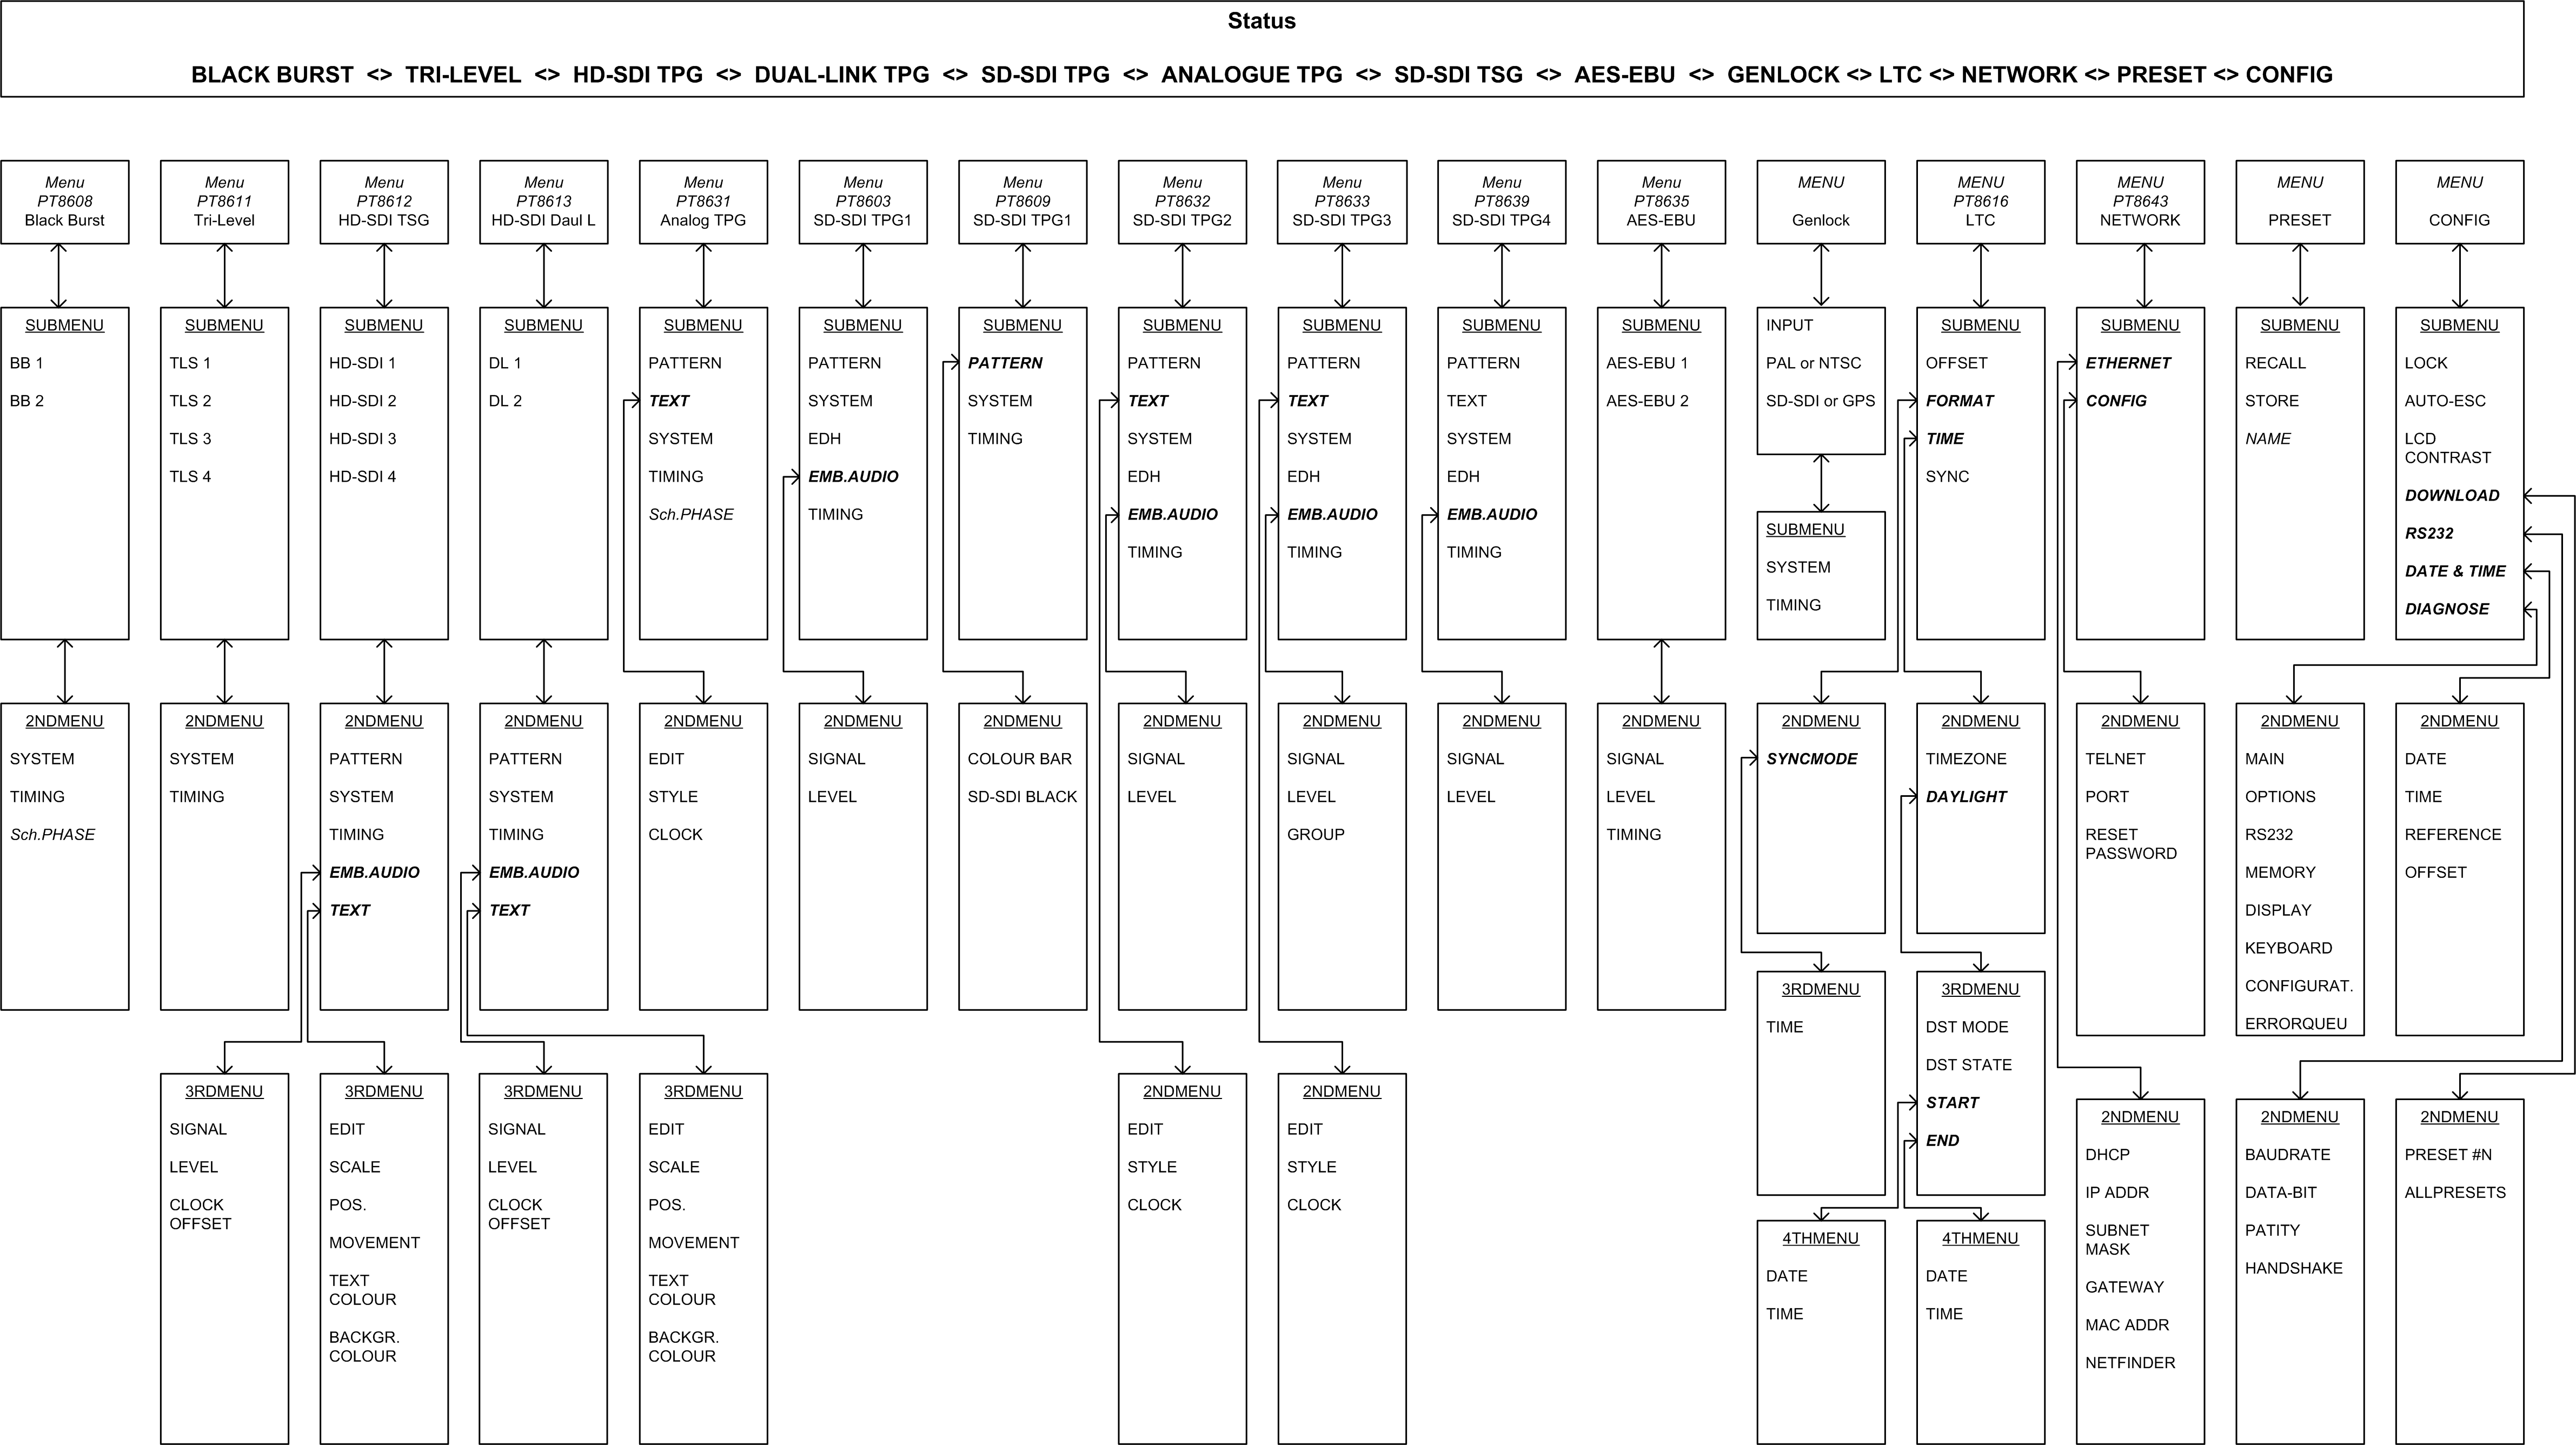
\includegraphics[width=1.25\textwidth]{fig/menu_tree}
	\caption{PT5300 Menu tree}
\end{figure}
\end{landscape}
\clearpage
